\documentclass{scutmaster}

\usepackage{pgf}
\usepackage{import}
\usepackage{graphicx}
\usepackage{booktabs}
\usepackage{multirow}
\usepackage{siunitx}
\usepackage{xcolor}
\usepackage{subcaption}
\usepackage[author={胡玮文}]{pdfcomment}
\usepackage{tikz}
\usepackage{wrapfig}
\usetikzlibrary{backgrounds,intersections,calc,positioning,fit,shapes.geometric}
\usepackage{hyperref}

\DeclareMathOperator*{\argmax}{arg\,max}
\DeclareMathOperator*{\argmin}{arg\,min}
\DeclareMathOperator{\sg}{sg}

\newcommand{\TODO}[1]{\textcolor{red}{TODO: #1}\GenericWarning{}{LaTeX Warning: TODO: #1}}

\title{基于可微分渲染的3D人脸重建方法研究}
\titleEN{3D Face Reconstruction Based on Differentiable~Rendering}
\date{\zhtoday}
\classificationnumber{TP391.41}

\author{胡玮文}
\authorEN{Weiwen Hu}
\studentnumber{202045611}
\phone{17701952145}
\email{sehuww@mail.scut.edu.cn}
\address{江西省南昌市青山湖区江大南路139号荣昌小区16栋(330029)}

\degree{电子信息硕士(软件工程)}{电子信息硕士}
\major{软件工程}{数字人}

\supervisor{杜卿}{副教授}
\supervisorEN{Assoc. Prof.}{Qing Du}

\school{软件学院}

\input{build/git_description}
\hypersetup{
    pdfinfo={
        Version=\gitdescription
    }
}

\begin{document}

\maketitle
\hideinblind{
    \maketitleEN
    \nominationpage
    \declareoforiginality
}

\frontmatter
\chapter{摘\texorpdfstring{\quad}{}要}

本文研究的3D人脸重建方法旨在从少量非受限环境拍摄的照片中恢复人脸的3D模型,
这些方法在计算机视觉、图形学和虚拟现实等领域都有广泛的应用。
其重建的模型已被广泛应用于人脸识别、人脸表情捕捉、人脸跟踪、人脸动画合成等任务中。
然而,现有基于少量非受限环境照片的重建方法流程复杂且精度有限,
尚难以直接应用于需要直接渲染图像的游戏、影视等场景中。
具体而言,现有方法未能充分利用照片中的边缘信息,它们依赖2D人脸关键点识别、多目立体等方法以重建人脸的几何形状,这增加了额外的复杂性和累积误差。
本文提出了一种基于可微渲染的新方法,旨在克服这些限制,显著降低了3D人脸重建流程的复杂度,提高了重建的精度。

为解决非受限环境照片中边缘信息难以利用的问题,
本文提出了一种基于可微分渲染的3D人脸重建算法。
本文从理论上分析了无法对背景准确建模时的可见性梯度计算问题,
提出了一种面积归一化的像素损失函数。
本文分析了该损失函数的作用机理,并与现有的通用可微分渲染研究中的可见性梯度计算方法相结合,高效实现了该损失函数。

然而人脸只是整个人体模型的一部分,当人脸模型被裁剪下来用于重建时,在人工裁剪的模型边缘会产生异常梯度。
为解决该问题,
本文进一步提出了一种基于SDF贴图的方法对所有渲染图像中的边缘进行分类,从而消除这些异常梯度,
最终使人脸3D模型能合理保持原有拓扑结构,从而提高了重建的准确性和实用性。

基于本文提出的这些方法,本文实现了一个基于逆渲染的完整自动化人脸重建流程。
该流程利用现有神经网络方法进行初始化,并结合传统方法重建人脸纹理。
其重建的人脸可在一定的视角、光照、表情变化下较为逼真的重新渲染。
本文展示和评估了其重建效果。

\keyword{关键词:} 可微分渲染;逆渲染;SDF贴图;人脸重建

\chapter{Abstract}

This thesis focuses on 3D face reconstruction methods that aim to recover 3D models of faces from a limited number of unconstrained photos.
These methods has a wide range of applications in various fields, including computer vision, graphics, and virtual reality.
Despite their widespread applications in areas such as face recognition, face expression capturing, face tracking, face animation synthesis, etc.,
current methods are complex and limited in accuracy.
In particular, existing methods fall short when it comes to directly rendering images in applications such as games and movies.
Specifically, the existing reconstruction methods do not fully utilize the edge information in the photos,
instead, they rely on 2D face landmark detection, multi-view stereo, etc.\ to reconstruct the geometric shape of the face,
which introduces additional complexity and cumulative error.
This thesis proposes a new approach based on differentiable rendering,
which promises to overcome these limitations and significantly reduce the complexity of the 3D face reconstruction pipeline,
as well as improve the accuracy of the reconstruction.

To address the challenge of leveraging edge information in unconstrained photos,
this thesis proposes a 3D face reconstruction algorithm based on differentiable rendering.
This thesis analyzes the difficulty  of computing visibility gradients in situations where the background cannot be accurately modeled,
and proposes an area-normalized pixel loss function.
This thesis analyzes the mechanism of this loss function,
and integrate it with the existing methods for computing visibility gradients in general differentiable rendering,
achieving an efficient implementation.

However, the face model is only part of the whole human model.
When the face model is cropped for reconstruction,
the artificial cut edges can produce abnormal gradients.
To overcome this issue, this thesis further proposes a method based on SDF maps to classify all edges in the rendered images,
which eliminates these abnormal gradients.
By ensuring that the reconstructed face model can reasonably preserves its original topology,
the proposed method enhances the accuracy and practicality of the reconstruction

Based on the proposed methods, This thesis presents a fully automatic face reconstruction pipeline based on inverse rendering.
The pipeline employs existing neural network methods for initialization and integrates traditional methods to reconstruct the face texture.
The resulting reconstructed face can be realistically re-rendered under certain views, lighting, and expression changes.
This thesis presents and evaluates the reconstruction results.

\keyword{Keywords:} Differentiable rendering; Face reconstruction; SDF maps; Face scanning

\tableofcontents

\listoffigures

\listoftables

\mainmatter
\chapter{绪论}
\label{chap:intro}

\section{研究背景}

3D人脸重建是计算机视觉和计算机图形学领域的一个热门研究方向。
相比于传统计算机视觉对2D照片的判断、识别和生成,3D人脸表示更加贴近实际,并可以建模光照和视角产生的影响。
例如,3D人脸模型可显式地表达人脸在3D空间中的位置,姿态甚至表情和骨骼的位置;
高质量的模型可用于逼真地一致地渲染出不同环境和视角下的人脸图像。

但相比于普通的摄影,3D人脸模型带来的优势是以更复杂的捕获过程为代价的,这通常会限制其应用范围。
直接捕获3D人脸信息通常需要立体视觉系统\citep{DEP,ss_geo}、3D激光扫描仪(如NextEngine和Cyberware)或RGB-D相机\citep{li2023}(如Kinect)。
前两种能捕获高质量的人脸扫描,但需要受控环境和昂贵的机器。
相比之下,RGB-D相机更便宜,更易于使用,但所得到的扫描质量有限。

在计算机图形学领域,
高质量的人脸模型已经可以用于在计算机中忠实地重现人脸,
包括角质层的凹凸、毛孔、皱纹、镜面反射和次表面散射等复杂特性。
这些模型已经在影视、游戏、动画、虚拟现实等领域中广泛应用,
但是其获取成本非常高昂。
目前成熟的影视级3D人脸重建方案仍是昂贵的商业解决方案,
其中包括大量复杂的步骤,并需要大量美术和技术人员参与制作\footnote{https://blog.unity.com/technology/making-of-the-heretic-digital-human-character-gawain}。
这些高精度重建方案通常使用专用设备在受控环境扫描的精细数据。
它们基于专业的摄影设备和完全受控的数据处理流程,
通过摄影测量的方法,使用相机作为测量仪器精确定量地测定各个方向上光线强度。
并基于较为准确的光学模型重建人脸的几何和材质。

相比之下,能从普通非受限环境的照片或视频中重建3D人脸模型的高效重建方法受到了广泛关注。
这类方法只需要最少单张手机随意拍摄的照片即可实时完成3D重建。
它结合了2D图像拍摄的便捷性和3D人脸模型的优势,
其应用非常广泛,目前已被用于人脸识别\citep{BlanzV03,1022631413.nh,zhu2015high}、人脸表情捕捉\cite{Mo2022TowardsAF}、人脸跟踪\citep{Pham2016RobustRP}、人脸动画合成\citep{Cao20133DSR,thies2016face2face}等任务中,并有代替人脸关键点识别等2D分析方法的潜力。

然而,该任务如今依然非常具有挑战性。
从少量非受限环境中拍摄的照片重建3D模型是高度不适定的。
算法需要从单张照片中估计出人脸几何形状、头部姿势和纹理、环境光照等参数,
参数空间很大,而不同解之间存在歧义,因为同一张照片可以从不同的3D模型中生成,
并且很难确定哪个模型才更加准确。
因此该任务必须结合有关人脸的先验知识才能完成。

基于人脸3D可形变模型(3D Morphable Model,简称3DMM)和神经网络的方法能以数据驱动的方式更好地建模有关人脸的先验知识。
3DMM是从大量人脸3D扫描中得到的统计模型,其先验知识通常编码于均值、方差等统计量中;
而神经网络则能从各种各样的监督信号中学习先验知识,例如3D模型、照片、关键点或高阶的人脸识别特征等。
这些先验知识有助于缓解3D重建的解之间的歧义。
在这些方法的加持下,我们虽然已经能高效地获得较为准确的3D人脸模型,
但这些模型都牺牲了大多数环境以及人脸表面上的细节,无法再次渲染从而忠实地还原照片,
因而并不能直接应用于影视,游戏等工业领域中。
另外,部分监督信号需要较为复杂的额外步骤才能得到,且可能引入额外的误差,
例如人脸关键点检测中,部分关键点的位置不论在照片或是在3D模型上都难以准确定义。
可以预见,在数字孪生和元宇宙等概念走入公众视野的今天,
基于现实的形象批量生产高渲染质量的人脸模型将涌现新的需求,
基于少量非受限环境照片的方便快捷的3D人脸重建技术具有重要现实意义。

在人脸重建方法中,可微分渲染技术已占有一席之地。
该技术旨在准确估计3D渲染结果关于其渲染参数(模型、光照等)的梯度,
从而引入直接的合成分析(Analysis by Synthesis)方法,也即逆渲染方法。
如今从模型渲染图片的过程已十分复杂,且随着计算机图形学和神经渲染等技术的发展还在不断进化,对人脸则更是如此。
而逆渲染方法直接将渲染结果和输入照片进行比较,根据渲染的误差来优化渲染参数,以此适应任意复杂的渲染方式。
可微分渲染则可以支持以简单的梯度下降法实现该优化过程,
具有通用、准确、自动化等优点,可谓是3D模型与2D照片之间的桥梁。
得益于此,基于非受限环境照片的高效重建方法得以直接从大量无标注的人脸照片的数据集中学习3D人脸模型的先验知识。
利用专业采集设备的高精度方案也因此获得更准确的材质参数。

然而,当前可微分渲染在人脸重建领域的应用还非常初步:
在渲染过程的梯度中,由于模型的不同部分之间相互遮挡而产生的可见性梯度通常最为显著,
这些梯度对模型与照片中的边缘的精确对齐至关重要。
但由于渲染采样过程的离散性,这些梯度往往难以估计。
在基于非受限环境照片的方法中,拍摄环境,相机参数,后处理流程等诸多不确定因素更提升了可见性梯度的估计难度。
现有人脸重建方法\citep{BFM,deep3d,DECA,bao2022}均仅考虑了逐像素着色的梯度,忽略了这些难以利用的可见性梯度,
这导致它们未能充分利用照片中的边缘信息,进而无法仅依赖可微分渲染来确定人脸的几何结构。
作为代替,现有方法依赖更加成熟的多目立体(multi-view stereo, MVS)或人脸关键点检测等方法。
但额外步骤将增加重建流程的复杂性,且导致误差在多个环节中累积。

综上,3D人脸重建技术应用广泛。
但现有高精度人脸重建方法所需数据采集环境要求高,实施困难。
在基于非受限环境照片的方法中,对可微分渲染的应用仍有待进一步发展。

\section{本文研究内容及贡献}

本文主要研究3D人脸重建方法的理论与应用。
本文提出了一套高精度多视角数据采集方案,解决了高精度人脸重建所需的数据采集环境要求高,实施困难的问题。
本文从可微分渲染在3D人脸重建中应用时遇到的实际问题出发,
提出了改进的理论,并在实践中验证了其有效性。
本文的主要贡献可概括如下:

\begin{enumerate}
\item 影视级真实的渲染效果离不开基于物理的渲染管线和精确的几何与材质数据。
若要获取这些数据,则需要精确的基于物理的测定。
本文提出了一套多视角人脸数据采集方案,
其旨在通过软硬件协同设计,对全流程的高精度控制,实现在精确的时间点、位置,高分辨率高精度地测定物体反射光线强度数据,
从而为基于物理的可微分渲染的优化提供坚实的基础。
本文介绍了该采集方案的软硬件设计,设备标定校准方法,使用交互方式和实现验证结果。

\item 针对可微分渲染在应用到3D人脸重建时,模型与背景交界处的可见性梯度难以被估计的问题,
本文从理论上分析了其原因是缺乏对背景的建模。
在缺乏对非受限环境中背景的先验知识的前提下,本文提出了面积归一化的像素损失,
以对可微分渲染的损失函数进行改进。
本文通过收缩、扩展两项梯度分析了其作用机理,
并提出了一种几乎无需额外计算和存储开销的方式实现这项改进。
本文通过实验证明了该项改进可以达成既定的目标:
在不对背景建模的情况下,使3D几何模型与照片中的物体边缘良好对齐。

\item 本文实现了一种通过单张在非受限环境中拍摄的照片,重建3D人脸模型的方案。
本文通过集成神经网络和3DMM人脸模型以提升鲁棒性;
通过可微分渲染技术实现更精准的对齐,
并在前述理论的基础上提出了一种基于SDF贴图的方法,消除了人工裁剪的边缘带来的异常梯度;
还集成一些传统算法以在3D模型上重现照片中的更多细节。
该方案中的逆渲染优化过程仅使用了像素损失函数,
以非常简单的流程实现了精确的边缘对齐。
取各家所长,该方案最终实现了细节丰富且全自动的,基于单张非受限环境照片的3D人脸模型重建。
其输出的3D人脸模型可支持在一定视角、光照和表情变化内较为逼真地重新渲染。

\end{enumerate}
本文的研究内容及其关系总结如图\ref{fig:structure}所示。

\begin{figure}[htb]
    \centering
    \begin{tikzpicture}[
        level 1/.style={sibling distance=7.7cm},
        level 2/.style={sibling distance=4.7cm, nodes={font=\small,draw}, align=center},
        level 4/.style={nodes={draw=none, font=\normalsize}},
        t/.style={align=center, text width=2em, font=\bf},
    ]
        \linespread{1.1}
        \node (title) {\bf 高精度3D人脸重建关键环境及可微分渲染技术研究}
        child {
            node (high) {使用专业设备的高精度方法}
            child {
                node (problem1) {采集环境要求高,实施困难}
                child {
                    node (content1) {多视角人脸数据采集方案}
                    child {node (chap3) {第\ref{chap:platform}章}}
                }
            }
        }
        child {
            node (efficient) {基于非受限环境照片的方法}
            child {
                node {未能充分利用照片中边缘信息}
                child {
                    node {适应未知背景的可微分逆渲染}
                    child {node (chap4) {第\ref{chap:method}章}}
                }
            }
            child {
                node {裁剪边缘的异常梯度}
                child {
                    node {人脸重建实现}
                    child {node (chap5) {第\ref{chap:recon}章}}
                }
            }
        };

        \node (t1) [t,left=5mm of problem1] {问题};
        \node at (content1 -| t1) [t] {研究内容};
        \node at (chap3 -| t1) [t] {对应章节};

        \path [->,draw] (chap4) -- node [above] {\small 应用} (chap5);
    \end{tikzpicture}
    \caption{本文的研究内容及其关系}
    \label{fig:structure}
\end{figure}

\section{本文组织结构}

本文正文共分为6个章节,各章节的主要内容如下:

\newcommand*{\chapref}[1]{\paragraph{\hyperref[{#1}]{第\ref*{#1}章 \nameref*{#1}}}}

\chapref{chap:intro}
本章介绍了3D人脸重建、以及可微分渲染的背景、关联及其研究意义,
并总结了本文主要贡献及各章节的内容安排。

\chapref{chap:related_work}
本章对课题相关的研究内容进行了综述,
其中包括使用专业设备的和非受限环境下的3D人脸重建、以及可微分渲染相关方向的研究和实践。
此外,还介绍了一些可用于3D人脸渲染的计算机图形学的基础知识。

\chapref{chap:platform}
为了更专业地采集基于物理的人脸渲染所需的材质数据,
本章介绍了一套多视角人脸数据采集方案。
该方案中定制的软硬件能够实现高分辨率人脸照片的便捷多视角采集,
并为后续的数据收集整理,相机、光源标定等重建所必备的步骤提供了软件支持。
本章将介绍该平台的软硬件设计思路、实现细节、使用方法以及其产出数据可能的应用。

\chapref{chap:method}
本章介绍了本文提出的一种对现有可微分渲染的改进方法。
该方法能增强可微分渲染技术在难以建模背景的图像拟合任务中的适应能力。
其理论构建在修改的损失函数之上,并通过收缩、扩展两项梯度项来实现。
本章也通过实验验证了该方法的有效性。

\chapref{chap:recon}
利用上一章提出的方法,本章介绍了一个从单张非受限环境照片重建3D人脸的实现。
该实现解决了人工裁剪的边缘处异常梯度的问题,
同时有机结合了神经网络、可微分渲染和一些传统算法,
达成了快速高效,细节丰富且全自动的3D人脸模型重建。
本章也与其他相关工作进行了比较。

\paragraph{\nameref{chap:conclusion}}
基于本文完成的工作结果对本文研究进行总结,并分析当前工作存在的不足和对未来工作的展望。


\chapter{相关研究综述}
\label{chap:related_work}

本章主要介绍本课题的相关研究和实践工作,
其中包括高精度的多视角3D重建方法,
基于少量数据的高效3D人脸重建方法,
可微分渲染以及它在人脸重建中的应用。

\section{多视角3D重建}

这类方法力求通过模型来精确描述被采集对象的形状和材质,从而在重新渲染时表现出很高的逼真度。
这些模型通常能从任意角度,在任意光照环境下重新渲染,以满足影视、游戏等领域的需要。

\paragraph{几何形状重建}
几何形状是物体最基本的属性,即物体每个部分在空间中所处的位置。
几何形状重建的基本原理是识别物体同一个部分在不同相机下的匹配关系,然后借助已知的相机参数,以及该部分在不同相机下的像素坐标,计算出该部分在3D空间中的坐标。称为基于视差的方法。

而计算机中描述几何形状的方法有很多种,其中最基本的是点云模型,它保存了大量位于物体表面的点的坐标。
这种表示也是大多数几何重建算法的目标。
最初,\citet{PFM}通过在目标脸上画一些网格,从而允许手动建立格点间的匹配关系,并建立稀疏的点云。
\citet{ss_geo}对多个相机两两之间计算视差图,然后将多组视差图进行融合,并通过约束进一步排除误匹配点,最终得到一个稠密的点云。其中视差图正是两张照片中,像素级别的匹配关系。视差图的构建是分辨率从低到高逐步细化的,并在过程中应用了平滑性、唯一性和顺序性的约束,以消除误匹配点。
这类方法统称为Multi-View Stereo (MVS)。
\citet{DEP}则利用投影仪在目标表面投影彩条图案,以使匹配结果更加鲁棒。
3dMD的商业3D重建解决方案\footnote{https://3dmd.com/}也使用了斑点图案的投影。
D3DFACS\citep{D3DFACS}数据集采用了3dMD的方案。
在匹配过程中,镜面反射的效果会随视角的变化而变化,从而导致匹配结果的不准确。
因此有不少方法\citep{DEP}选择使用偏振将镜面反射的效果去除,从而提高匹配的准确度。
但由于次表面散射的存在,这种方法得到的几何形状会过于平滑。但这或许不是一个问题,因为在后续估计材质的过程中,会再估计更高分辨率的法向。

虽然视差仍然是最广泛使用的方法,其准确度也非常高,但也不乏其他可行的方法。
例如,\citet{MaHPCWD07}使用光度立体的方法,通过多种球面梯度偏振光源的成像效果,重建物体的表面法向。高分辨率的法向信息可与中等分辨率的结构光的结果进行融合,从而获得高分辨率的几何形状,且能避免单纯依靠法线积分带来的累积误差。
\citet{phase_shift}则将相移方法与视差结合,以获得更高的准确度和鲁棒性。
\citet{BJUT3D}选择使用激光扫描仪。
FaceWarehouse\citep{FaceWarehouse}数据集采用了Kinect深度相机。

在得到点云之后,还需要将点云转换为网格,
该网格的拓扑结构应在采集的不同帧间,以及不同人物间保持一致,
以供渲染、人工编辑,动画制作等使用。
该任务的重点在于找到不同帧间的点的匹配关系,从而重建人脸的运动,变形等特征。
很多方法\citep{PFM,DEP,BickelBAMOPG07}通过在脸上画上易于识别的标记点以辅助匹配。但画标记点将给采集带来额外的麻烦,且会影响到之后人脸材质的估计。
\citet{BeelerHBBBGSG11}通过图像空间跟踪和锚点帧的方法,获取稠密且累积误差小的匹配关系,从而将网格的拓扑结构传播到所有帧,再逐帧根据点云进行微调。
FLAME\citep{FLAME}则完全依靠3D数据,而不使用照片。FLAME是一个由少量PCA得出的参数控制的3D网格模型。它交替地训练该模型和将该配准到3D数据上,从而找到3D数据间的匹配关系。
但3D数据中所包含的信息量有限,因此完全依靠3D的数据的理论精度应不如跟踪图像的方法。
也有一些方法能直接从照片中重建网格,而不需要先得到点云。
\citet{LiLBL0Z21}以传统方法的结果为训练数据,训练一个神经网络,通过体素特征,由粗到细地直接生成网格。

近年来,随着神经辐射场(NeRF)\citep{nerf}等技术的发展,也有一些方法将几何形状编码在神经网络等隐式表达中,而不使用点云、网格等显式表达。
NeRF\citep{nerf}首先提出将几何信息编码在用神经网络表示的密度场中,然后通过体渲染的方法,将渲染结果直接与照片比较,从而优化该模型。
然而,这类隐式模型虽然构建简单,但有诸多问题,例如难以进一步人工编辑,渲染效率较低等。
\citet{MoRF}通过神经网络生成的形变场以表示人脸几何形状,从而将几何形状和材质分离,提升了可编辑的程度。
\citet{nvdiffrec,nvdiffrecmc}先优化在可变形四面体网格中存储的有向距离场,然后将其转换为传统的显式三角形网格,并使用可微分渲染进一步优化。以此解决隐式模型不易编辑的问题。

\paragraph{相机标定}
精确的相机标定是精确的多视角3D重建的基础。
目前主流的标定方法是用相机拍摄特制的标定目标。
\citet{ss_geo}采用在一个球形目标物体上随机地粘贴一些可识别的角点。
其优势在于不同角度下都能观察到较多角度较正的角点。
\citet{del_grid}提出使用三角形网格代替正方形网格,以在角点处提供更多的梯度信息,从而提升角点定位的精度。
\citet{SchopsLPS20}提出使用大量参数来描述相机模型,且大幅提升标定目标中角点的数量和角点中的梯度信息,从而更精确地估计这些参数。

\paragraph{材质估计}
材质指的是物体的表面法向、颜色、粗糙度、金属度、次表面散射等属性。
更宽泛地说,材质描述了物体将如何与光线相互作用。即如何吸收,折射,反射,散射入射的光线。
若要获得高质量的,可在任意光照条件下渲染的3D模型,则必须对材质进行建模并估计模型参数。

在采集时直接收集多种不同光照条件下的照片的方法称为主动光源方法。
第一代Light Stage\citep{light_stage}使用一个可绕人脸自动旋转的光源,从而获得人脸对各个方向入射光的响应情况,从而实现任意光照条件下的渲染。
此外,该作者还利用色彩空间分析技术\cite{temporal_color}对脸部的法线分布,颜色等属性进行建模,从而实现了任意视角下的渲染。该方法的缺陷在于其单帧图像的采集时间较长。
\citet{MaHPCWD07}通过LED阵列实现的偏振球面梯度照明将所需采集的照片数量减少到了8张,耗时也大幅减少。该方法也通过混合法向模型获得了较为真实的渲染效果,尽管在原理上不太符合物理模型。
此后\citet{KampourisZG18}进一步提出使用球面二值照明和色彩空间分析\cite{MallickZKB05}以分离镜面反射。同时该方法进一步减少了所需采集的照片数量。
\citet{FyffeGTGD16}的方案与本文的方案更为类似。该方法使用了6盏闪光灯并依次在几十毫秒内触发,并用24台相机分布在不同闪光灯闪光时触发快门。该方法可以在近乎瞬间完成采集,从而避免了被采集对象可能的运动。

与之相对的是被动光源方法,即在采集时光照条件保持不变。这类方法的硬件实现通常更为简单。但缺失的信息则需要通过多视角或者更强的正则化等来弥补。
\citet{RiviereGBGB20}使用了带有次表面散射的材质模型,分别采集了不同偏振方向的数据以更好地分离镜面反射和次表面散射。该方法实现了纹理空间的可微分渲染以估计模型中的参数。
在此基础上,\citet{XuRZCBG22}使用了更准确的偏振模型,光源模型,并建模了部分间接照明效果,使估计的材质参数更加准确。
\citet{nvdiffrec}使用通用的粗糙度-金属度材质模型,利用可微分光栅化渲染技术,联合优化模型的几何形状和材质参数。由于联合优化的难度较高,该方法需要大量的视角作为输入。

除了这些直接描述物理性质的参数化材质模型外,也有研究希望能使用神经网络作为材质模型。
例如NeRF\citep{nerf}也可建模并输出物体反射光线的颜色和强度,且可以建模反射随视角变化的变化,但无法建模与采集时不同的光照条件下的反射情况。

\section{高效3D人脸重建}

尺度正确\citet{ZielonkaBT22}

\section{可微分渲染}

\section{高质量人脸3D渲染}

\paragraph{基于物理的渲染}

\paragraph{分离求和近似}

\paragraph{次表面散射}


\chapter{适应未知背景的可微分逆渲染方法}
\label{chap:method}

在将可微分渲染方法应用到3D人脸重建任务时,现有方法均未能充分利用可见性梯度。
而该梯度正是所有梯度中的主要分量,对模型与照片的精确对齐有着重要作用。
通常来说,计算正确的可见性梯度需要同时具有前景和背景的模型,而在自然环境照片中,由于背景多样,很难得到显式的背景模型。
本章主要针对该问题,提出一种适应未知背景的可微分渲染方法,能够利用可见性梯度来优化模型与照片的对齐。

\section{问题定义}

可微分渲染旨在从参数化的3D模型,如三角形面片,纹理贴图等,渲染得到2D图片,同时计算该渲染结果关于其输入参数的梯度。
然后可以优化渲染结果与照片间的误差,以期利用基于梯度的方法优化输入参数,从而改善渲染效果,使之更加接近现实。
其在3D人脸重建的相关任务中已有较广泛的应用。

然而现有方法存在一些不足:
现有可微分渲染技术大多是对整张图片估计梯度,即不区分前景和背景部分。
但是,在基于自然环境照片的人脸重建任务中,我们通常只有前景(即人脸)的3D模型,而没有背景的模型。
此时,现有方法选择忽略模型间相互遮挡产生的可见性梯度,而这会造成模型与照片的对齐不准确,如图\ref{fig:problem_a}所示。
另一方面,若对背景进行很粗糙的建模,例如假设为全黑,则错误的梯度会导致模型无法正确收敛,如图\ref{fig:problem_b}所示。

\begin{figure}
\centering
\begin{subfigure}[t]{0.45\textwidth}
    \centering
    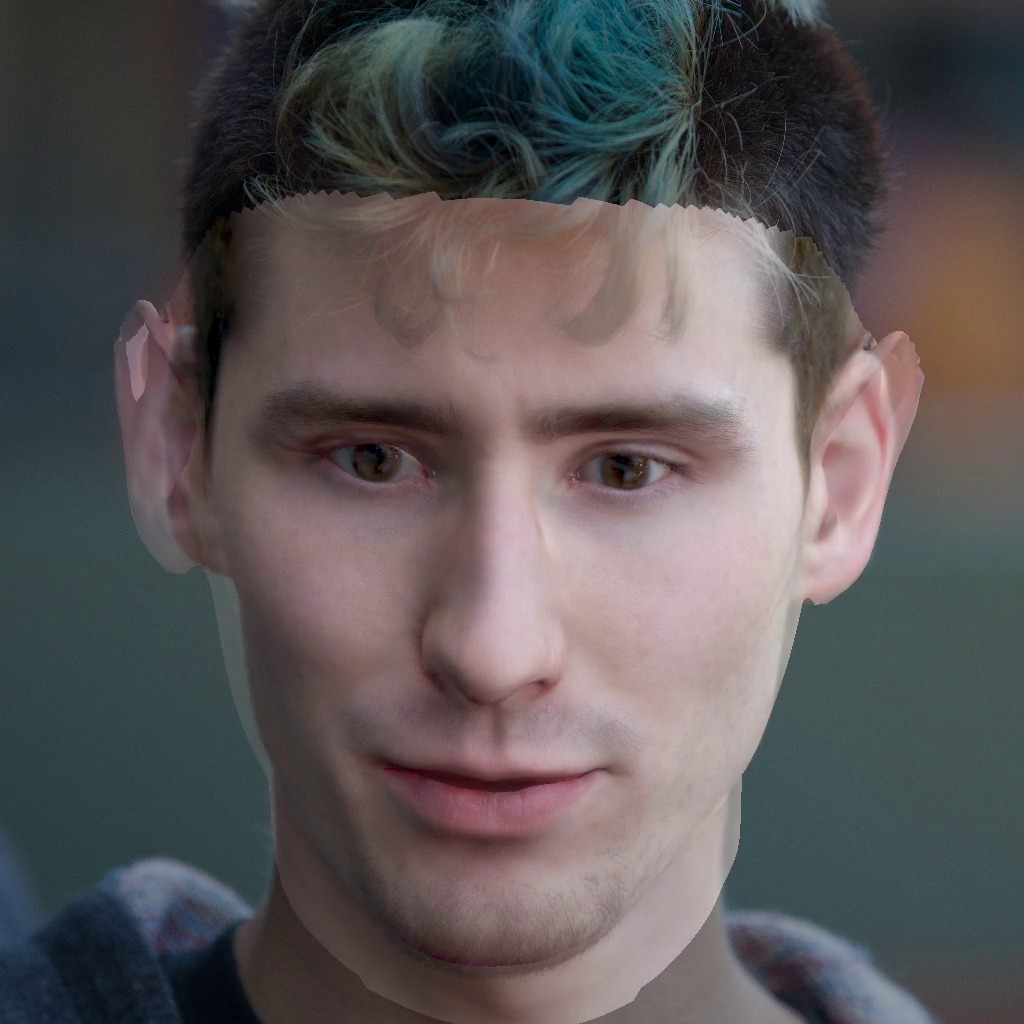
\includegraphics[width=\textwidth]{figures/black-bg_no-aa}
    \caption{忽略可见性梯度,模型与照片未准确对齐}
    \label{fig:problem_a}
\end{subfigure}
\begin{subfigure}[t]{0.45\textwidth}
    \centering
    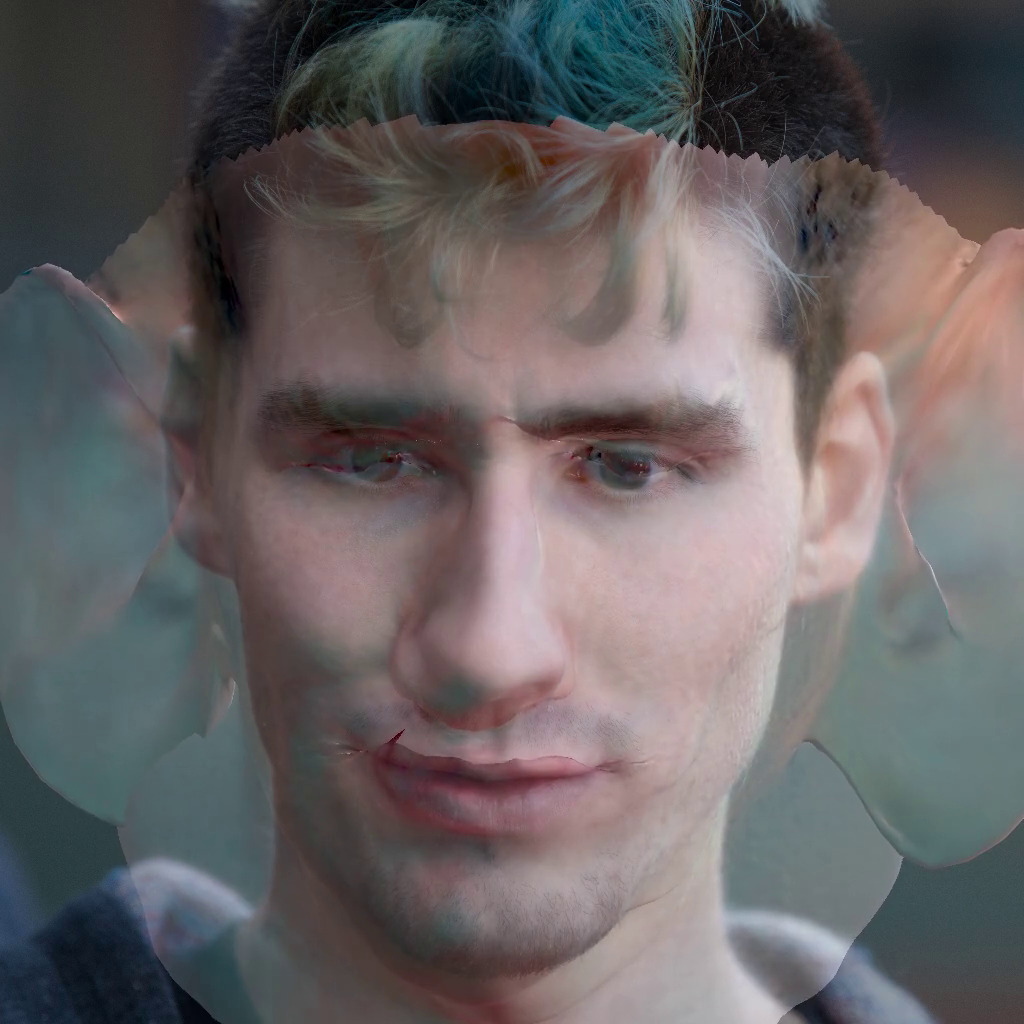
\includegraphics[width=\textwidth]{figures/black-bg}
    \caption{使用全黑代替背景模型,可见性梯度错误}
    \label{fig:problem_b}
\end{subfigure}
\caption[未知背景条件下可微分渲染优化结果]{
    未知背景条件下可微分渲染优化结果。
    示意图为目标照片和渲染结果以1:1 alpha混合后,再进行gammar校正得到。
}
\end{figure}

为绕过上述问题,现有方法通常:
使用多目立体等其他手段事先确定高精度的人脸几何形状,并在逆渲染优化过程中使几何形状保持不变\citep{RiviereGBGB20};
忽略可见性梯度,使用2D人脸关键点\citep{deep3d}、图像分割\citep{nvdiffrec}结果等辅助监督信息来补足这部分缺失的梯度。
但是,如果能够直接利用可见性梯度,可大大简化算法的流程,同时也能避免在前序步骤中引入额外的误差。

本节将设计一个简单的玩具实验来更直观地说明上述问题。
如图\ref{fig:problem}所示,我们使用一个简单的白色平面作为前景模型,用其拟合一个白色青色对半分割的场景。
该模型的参数是其横向的平移量,用平面边缘与横坐标轴的交点$a_x$表示。
该平面的边缘稍微倾斜,以突出可见性梯度的变化。
该平面的着色不受参数影响,始终固定为白色。
该例子中使用的损失函数为L1误差,即:
\begin{equation}
\mathcal{L} = \left\| \hat{\mathcal{I}} - \mathcal{I} \right\|_1
\text{。}
\label{eq:loss_l1}
\end{equation}

\begin{figure}
\centering
\import{build/figures}{problem.pgf}
\caption[在未知背景时计算可见性梯度困难]{
    在未知背景时计算可见性梯度困难。
    拟合目标和渲染结果左侧白色为前景,右侧为背景。
    前景模型为以红线为边界的白色平面。
    横坐标为前景模型的平移量。
    函数值为每像素均匀采样65536次的数值近似。
    (a)离散采样,不计算可见性梯度;
    (b)使用不准确的黑色背景模型计算可见性梯度,模型无法收敛到期望位置;
    (c)理想情况下,在完全已知背景时的可见性梯度,模型能准确收敛至梯度为0的点。
}
\label{fig:problem}
\end{figure}

其中,(a)为离散采样的方式,也是目前大多人脸重建中使用的方法。
其渲染流程为:在每个像素的中点处采样,若其位于前景模型的覆盖范围内,则渲染为白色,否则渲染为背景。
由于采样过程是离散的,且$a_x$的改变并不会影响采样的模式,因此,渲染结果$\hat{\mathcal{I}}$关于$a_x$的梯度为0,其损失函数为阶梯函数。
即该损失函数完全无法以基于梯度的方式指导模型拟合。

另一方面,在没有准确背景模型的前提向,可见性梯度则难以被利用。
例如,在(b)中,假设我们并不知道该场景的背景,因此直接假设其为全黑。
但在本例中这个假设显然是不准确的。
(b)和(c)的渲染方式与(a)不同,其每个像素的颜色取决于前景模型覆盖该像素的面积的比例,并按面积比例线性混合前景和背景的颜色。
这使得处于前景边缘处的像素的颜色成为了关于$a_x$的连续函数,即产生了所谓的可见性梯度。
在此前提下,从图中可以观察到其损失函数呈递减的趋势,并未在期望的位置上形成极值。
因此,该梯度也无法引导模型收敛到期望的位置。

作为参考,(c)展示了理想中,完全已知背景的情况下,可见性梯度的作用。
从图中可见,其损失函数在期望的位置上有一个明显的极值,且其周围的梯度将能很好地指导优化器,使模型收敛到该位置。

然而,在实际人脸重建的任务中,特别是从自然环境照片的重建中,背景可能是很复杂且难以建模的。
本章将探讨如何在这种情况下,如何利用可见性梯度以指导前景模型与目标照片对齐。

\section{面积归一化的像素损失函数}

在分析中,不妨先将目标照片$\hat{\mathcal{I}}$和渲染结果$\mathcal{I}$抽象为连续的颜色场$\mathbb{R}^2 \to \mathbb{R}^3$。
于是公式\ref{eq:loss_l1}中的原始L1损失函数可改写为:
\begin{equation}
\mathcal{L} = \iint_{\mathcal{A}} \left\| \hat{\mathcal{I}} - \mathcal{I} \right\|_1 \mathrm{d}\sigma +
\iint_{\mathcal{B}} \left\| \hat{\mathcal{I}} - \mathcal{I} \right\|_1 \mathrm{d}\sigma
\text{,}
\label{eq:loss_l1_area}
\end{equation}
其中,$\mathcal{A}$为渲染结果中前景模型覆盖的区域,$\mathcal{B}$为背景覆盖的区域。
由此我们可以对图\ref{fig:problem}b中的现象进一步地解释:
当前景模型的边界向右移动越过中点之后,由于不能很好地拟合背景,该损失函数的第一项开始上升,这是符合预期的。
但是,由于采用的背景模型不准确,背景部分也存在一定误差,且由于背景区域面积下降,损失函数的第二项将会下降。
这两项相互制衡,导致前景和背景模型“抢夺”处于交界处的像素。
若背景模型的误差足够大,以至于使用前景模型来拟合背景区域反而占优势,则会出现如b)中的现象:前景模型将在优化中不断抢占背景的区域,从而无法收敛到期望的位置。
在实际中这种情况是很有可能的,比如在3D人脸重建中,人脸的材质模型通常具有很高的自由度以拟合人脸的细节,这些自由度可能被误用于拟合背景。

为解决在未知背景下的逆渲染问题,本文提出了一种面积归一化的像素损失函数:
\begin{equation}
\mathcal{L}_n = \frac{\iint_{\mathcal{A}} \left\| \hat{\mathcal{I}} - \mathcal{I} \right\|_1 \mathrm{d}\sigma}
{\iint_{\mathcal{A}}\mathrm{d}\sigma}
-\alpha\iint_{\mathcal{A}}\mathrm{d}\sigma
\text{。}
\label{eq:loss_n}
\end{equation}
该损失函数仅在前景模型覆盖的区域内计算损失,因此不会受到背景模型的误差影响。
该函数第一项为单位前景区域面积内的平均误差,第二项鼓励更大的前景区域,$\alpha$为一个超参数。

\begin{figure}
\centering
\import{build/figures}{one_dim_loss.pgf}
\caption{面积归一化的像素损失函数在一维的作用分析}
\label{fig:one_dim_loss}
\end{figure}

为了更好地理解该损失函数的作用,本文将展示一个一维情况下的简单例子。
如图\ref{fig:one_dim_loss}a所示,假设拟合目标包含前景和背景,为阶跃函数;前景模型为定义在前景区域$\mathcal{A}=(0,\theta)$的常函数,$\theta$为模型参数:
\begin{align}
\mathcal{I}(x) &= \begin{cases}
    1   & x \leq 0.6 \\
    0.1 & x > 0.6
\end{cases}\\
\hat{\mathcal{I}}(x) &= 0.8 \quad x < \theta
\text{。}
\end{align}
在此定义下,我们可求出$\mathcal{L}_n(\theta)$中各项的解析表达式:
\begin{align}
\int_{\mathcal{A}} \left\| \hat{\mathcal{I}} - \mathcal{I} \right\|_1 \mathrm{d}\sigma
&= \int_0^{\theta} \left| \hat{\mathcal{I}}(x) - \mathcal{I}(x) \right| \mathrm{d}x \\
\int_{\mathcal{A}}\mathrm{d}\sigma &= \int_0^{\theta} \mathrm{d}x = \theta
\text{。}
\end{align}
其函数图像如图\ref{fig:one_dim_loss}b、c、d所示。
该函数第一项的分子为公式\ref{eq:loss_l1_area}中的第一项前景部分,显然该项是随着$\theta$单调递增的。
由于没有了背景部分的制衡,单独使用该项将导致模型收敛到一个很小的区域。
于是本文将该项以前景区域的面积进行归一化,即$\mathcal{L}_n$的第一项。
若该模型的拟合误差在前景区域内是均匀分布的,则该项将会是一个常数,不会引导模型减小面积。
而模型拟合背景区域的误差通常显著大于拟合前景,因此该项鼓励模型离开背景区域,从而减小平均误差。
而在当前景区域小于期望时,$\mathcal{L}_n$的第二项将会鼓励模型增大面积,准确对齐到目标的边界上。如图d)所示,$\mathcal{L}_n$在$\theta=0.6$处取得极值,此时模型的前景区域正好对齐了目标的边界。
同时,若有拟合误差在边缘处大于中心的情况,第二项也能提供一定的补偿。
直观地,若拟合目标具有清晰的边界,且在边界处模型拟合前景的误差小于拟合背景的误差,则存在一个$\alpha$,使模型能精确对齐到该边界上。

推广到二维的情况会稍微复杂,因为在二维下边界不止一个点,而边界的不同位置将会有不同情况。但根据以上分析,本章提出的损失函数最适用于以下场景:
\begin{enumerate*}
    \item 背景复杂且未知,但拟合目标具有清晰的边界;
    \item 在前景物体边界附近的拟合误差不显著高于中心区域;
    \item 在边界上,模型拟合前景的误差小于拟合背景的误差。
\end{enumerate*}
若在边界的个别区段上不能满足上述条件,则需要通过一定的平滑等正则化方法进行补偿。
常见的情况比如:
由于景深浅,照片中物体边缘有较大模糊;
或者在部分位置碰巧前景与背景颜色相似等。

\section{收缩\&扩展梯度}

本节将介绍如何将上一节提出的,定义在连续空间的损失函数应用于由离散的像素组成的图像上,并最终实现为收缩和扩展两项梯度的形式。

为了使损失函数成为关于渲染图像$\hat{\mathcal{I}}$的l连续函数,我们将图像渲染的过程定义为:
\begin{equation}
\hat{\mathcal{I}}(x,y;\theta) \to (\mathbf{c}, \sigma) \quad x,y \in \mathbb{Z}
\text{。}
\end{equation}
其中$x,y$为像素坐标,$\theta$为前景模型的参数,$\mathbf{c}\in\mathbb{R}^3$为着色后的像素颜色,且对模型覆盖区域外的像素没有定义,$\sigma\in[0,1]$为前景模型覆盖该像素的覆盖率,即该像素中被模型覆盖的面积占其总面积的比例。
$\mathbf{c}$的值取决于所选择的着色模型,因此在本章中不考虑其关于$\theta$的梯度。
自然地,对于处在模型内部的像素$\sigma=1$,而对于模型外部的像素$\sigma=0$,
仅当像素位于模型边界上时,$\frac{\partial\sigma}{\partial\theta}$才不为0,因此处于模型边界上的覆盖率$\sigma$是本节主要考虑的对象。
需要注意的是,准确地求出每个像素的$\sigma$运算量较大,后文第\ref{sec:method_discuss}节将介绍一种实现方式。

基于该定义,我们可以将面积归一化的像素损失函数的定义推广至由离散的像素表示的图像中:
\begin{equation}
\mathcal{L}_n = \frac{\sum_{x,y} \sigma \left\| \mathbf{c} - \mathcal{I} \right\|_1}
{\sum_{x,y} \sigma} - \alpha \sum_{x,y} \sigma
\text{。}
\label{eq:loss_n_pixel}
\end{equation}
与之前定义在连续空间的公式\ref{eq:loss_n}相比,该定义假设了同一个像素范围内的图像颜色保持不变。

下面将对该损失函数的梯度进行分析,以探寻其性质和可能的实现方式。
对公式\ref{eq:loss_n_pixel}求导可得:
\begin{equation}
\frac{\partial\mathcal{L}_n}{\partial\theta} =
\sum_{x,y}\left[
    \frac{
        \overbrace{\left\| \mathbf{c} - \mathcal{I} \right\|_1 \sum\sigma}^\text{收缩} -
        \overbrace{\sum \sigma \left\| \mathbf{c} - \mathcal{I} \right\|_1}^\text{扩展}
    }{\displaystyle\left(\sum\sigma\right)^2} - \alpha
\right]\frac{\partial\sigma}{\partial\theta}
\text{。}
\end{equation}
注意在该推导中我们忽略了$\mathbf{c}$关于$\theta$的梯度,这项梯度由具体的着色模型确定,通常可以使用自动微分求得。
从该推导结果中可以发现以下特点:
\begin{enumerate*}
    \item 该梯度仅在$\frac{\partial\sigma}{\partial\theta}$不为0时才不为0,因此在计算时仅需考虑处于前景模型边界上的像素;
    \item 其大体可分为收缩和扩展两项,分别将鼓励模型向内收缩其边界和向外扩展其边界;
    \item 当模型边界进入背景区域时,收缩梯度由于边界处误差较大而较大,但扩展梯度由于只依赖于平均误差,因此上升幅度较小,此时收缩梯度将占主导地位,鼓励模型离开背景区域;
    \item 若拟合误差分布均匀,即$\left\|\mathbf{c} - \mathcal{I}\right\|_1$与$x,y$无关,则收缩和扩展两项梯度相等,此时$\alpha$将轻微地鼓励扩展,以对齐边界。
\end{enumerate*}
这些特点均和之前的连续空间定义的损失函数相同。

虽然可以直接根据公式\ref{eq:loss_n_pixel}使用自动微分计算梯度,
但其中的覆盖率$\sigma$仅在模型边界上才不为0,其余部分的$\sigma$并不需要保存到内存中。因此我们可以实现以下损失函数:
\begin{equation}
\tilde{\mathcal{L}}_n =
\underbrace{\frac{1}{|\mathcal{A}|}\sum_{x,y|\sigma\in(0,1)} \sigma\left\| \mathbf{c} - \mathcal{I} \right\|_1}_{\text{收缩}} -
\underbrace{\left[\frac{\sum\left\| \mathbf{c} - \mathcal{I} \right\|_1}{|\mathcal{A}|^2}+\alpha\right]\sum_{x,y|\sigma\in(0,1)} \sigma}_{\text{扩展}}
\text{,}
\label{eq:loss_n_tilde}
\end{equation}
其中$|\mathcal{A}|$为优化开始时前景模型覆盖的面积,即$\sum_{x,y} \sigma$。
由于基于梯度的逆渲染方法通常并不能处理大范围的模型移动,因此该项可以近似看作常数。
该式也假设了边缘区域相对于整张图片来说是很小的。
由于该式仅对边缘区域计算,其关于$\mathbf{c}$的梯度也可以忽略。
注意此处列出的$\tilde{\mathcal{L}}_n$仅包含了模型与背景间的可见性相关梯度,在实际中需要配合通常的可微分渲染以计算颜色$\mathbf{c}$和其他已知背景的可见性梯度。

根据以上分析,我们最终得到了一个附加的,仅定义在模型边缘处像素的损失函数。
该函数的目的是在逆渲染的优化中,产生额外的收缩与扩张两项梯度,从而促进模型对齐到与未知的背景的边缘。

\section{实验结果}

\TODO{随机背景方块重建}

\section{讨论}
\label{sec:method_discuss}

\paragraph{基于nvdiffrast的实现}
本文基于上文所述理论,基于nvdiffrast\citep{nvdiffrast}中的抗锯齿模块进行了实现。

\begin{figure}
    \centering
    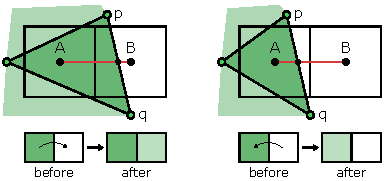
\includegraphics{figures/antialias}
    \caption[nvdiffrast抗锯齿模块的工作流程]{nvdiffrast抗锯齿模块的工作流程\citep{nvdiffrast}。}
    \label{fig:aa}
\end{figure}

为了完整性,这里简要介绍该模块的作用。
如图\ref{fig:aa}所示,该模块修改过的像素为左图的B和右图的A。
其中绿色的部分覆盖该像素的面积占整个像素面积的比例为覆盖率$\sigma$。
记修改前绿色部分的像素值为$\mathbf{c}$,白色背景的像素值为$\mathcal{J}$。
则修改后的像素值为:
\begin{equation}
\mathbf{c}' = \sigma\mathbf{c} + (1-\sigma)\mathcal{J}
\text{。}
\end{equation}

基于该模块,本文使用目标图像$\mathcal{I}$作为背景进行渲染,即$\mathcal{J}=\mathcal{I}$,则公式\ref{eq:loss_n_tilde}中的收缩项可进一步表示为:
\begin{equation}
\sigma\left\| \mathbf{c} - \mathcal{I} \right\|_1 =
\left\| \sigma\mathbf{c} + (1-\sigma)\mathcal{I} - \mathcal{I} \right\|_1 =
\left\| \mathbf{c}' - \mathcal{I} \right\|_1
\text{。}
\label{eq:impl_nvdiffrast}
\end{equation}
如此便可将收缩项中的$\sigma$完全交给该抗锯齿模块处理,且几乎没有额外的计算量。
更好的是,在同一抗锯齿模块中还可以同时处理其他已知背景部分的可见性梯度,例如下巴和脖子间,鼻子和脸颊间。

但nvdiffrast的覆盖率计算是稀疏的,即有部分$\sigma\in(0,1)$的像素无法被检测到,检测的概率和所用3D模型的网格密度有关。
而扩张项的梯度与收缩项相互制衡,因此其梯度的计算必须与收缩项相互耦合,即他们稀疏的模式必须相同
又注意到扩张项的梯度对于边缘的每一个像素是均匀的,因此本实现直接在反向传播时,对所有实际检测到$\sigma\in(0,1)$的像素添加上该项梯度。该方法也基本无额外内存和运算开销。

nvdiffrast的稀疏覆盖率检测有时会导致整体梯度估计的偏差过大,进而导致模型不能收敛到期望的位置,
因此可能还需要手动将相关梯度乘以一个放大系数进行补偿。
下文将对该问题进一步讨论,并提出另一种缓解措施。

\paragraph{L1距离的必要性}
本文中所有的讨论都是基于渲染图像与目标图像的L1距离的,之所以不使用L2或其他距离,主要是基于以下原因:
\begin{itemize}
\item 直接的原因是公式\ref{eq:impl_nvdiffrast}中$\sigma$和求距离的运算的交换需要L1距离。
\item 根本的原因是若将图像看作二维连续函数的离散化,则离散化的操作应尽可能小地对优化造成影响。
使用L1距离才能实现与像素离散化的方式无关的可见性梯度。
如图\ref{fig:problem}c所示,虽然该例子中图像分辨率很低,但其损失函数的梯度仍然是非常平滑的,并未受到像素离散化的影响。
图\ref{fig:l2_loss}展示了另一个使用L2损失的玩具实验的效果。
可见其梯度在像素边缘处出现了明显的阶跃,这是由像素离散化造成的。甚至在像素边缘处得到了为0的梯度,这显然是不合理且不利于优化的。
\end{itemize}

\begin{figure}
    \centering
    \import{build/figures}{l2_loss.pgf}
    \caption[L2损失与像素离散化相关]{L2损失与像素离散化相关,各图含义参见图\ref{fig:problem}。}
    \label{fig:l2_loss}
\end{figure}

\paragraph{nvdiffrast可见性梯度稀疏的缓解}
前文提到,nvdiffrast的抗锯齿模块计算的覆盖率是稀疏的,即它会错过部分$\sigma\in(0,1)$的像素。
该问题的原因在于其检测渲染图像中不连续性(即包含前景和背景相互遮挡)的方式。
该模块判定相邻两个像素不连续,当且仅当:
\begin{enumerate*}
\item 两个像素渲染自不同的三角形;
\item 其中来自前景的(深度较浅的)三角形在相机视角中处于物体边缘。
\end{enumerate*}
其中,处于边缘的判定方法为:来自前景的三角形满足以下条件之一:
\begin{enumerate*}
\item 在背景方向上无与其相邻的三角形;
\item 在背景方向上与其相邻的三角形朝向相机背面。
\end{enumerate*}
然而,真正处于边缘的三角形可能并未被渲染图像的任何一个像素采样到。
处于边缘的三角形被采样到的概率正比于其在渲染图像上的投影面积。
但为了提升精度而使用更高密度的网格会导致每个三角形面积的下降;
更雪上加霜的是,位于边缘的三角形的法向通常与相机方向夹角很大,导致其在渲染图像上的投影面积更小。
最终导致即使使用很高的分辨率也无法实现令人满意的采样概率。

为缓解该问题,本文提出放松处于边缘的判定条件,添加一条:背景未被任何三角形覆盖。
在该条件下即可保证与未知背景交界的所有边缘均被检测到。
但付出的代价是部分梯度不能正确地传递到真正处于边缘的顶点上,
而是被传递到与边缘相近的真正被采样到的三角形的顶点上。
但是在完整的优化问题中通常都具有鼓励模型局部光滑的正则项,这些梯度的影响最终将被较为均匀地分布到更大的区域上,因此这些偏差应该不会造成太大的影响。
图\ref{fig:vis_grad}展示了一些具体的例子。

此外,该方法只能缓解模型与未知背景间的不连续性判定,而对模型自身不同部分的遮挡无能为力。
这会导致内部的可见性梯度偏小,从而导致整体梯度估计发生偏差。
其具体影响需根据实际应用进一步分析。

\begin{figure}
    \centering
    \begin{subfigure}{0.33\textwidth}
        \centering
        \begin{tikzpicture}
            \path[use as bounding box] (-0.5,-0.5) rectangle (4,2.5);
            \draw [help lines] (0,0) grid [step=2cm] (4,2);
            \draw[red, name path=H] (1,1) -- (3,1);
            \filldraw (1,1) circle (1pt) node [above] {A}
                      (3,1) circle (1pt) node [above] {B};

            \coordinate [label=right:p] (p) at (1.2,2.2);
            \coordinate [label=right:q] (q) at (2,-0.3);
            \coordinate (r) at (-0.5,1);

            \draw (p) -- (r) -- (q);
            \draw [green!30!black, name path=T, thick] (p) -- (q);
            \path [name intersections={of=H and T,by=I}];

            \draw[fill=green] (p) circle (2pt);
            \draw[fill=green] (q) circle (2pt);
            \draw[fill] (I) circle (1pt);

            \begin{pgfonlayer}{background}
                \fill[green!50] (p) -- (1.1, 2.5) -- (-0.5,2.5) -- (-0.5,-0.3) --  (-0.5,-0.5) -- (2, -0.5) -- (q);
                \fill[green!80!black] (p) -- (q) -- (r) -- cycle;
            \end{pgfonlayer}
        \end{tikzpicture}
        \caption{正常检测到的边缘}
    \end{subfigure}%
    \begin{subfigure}{0.33\textwidth}
        \centering
        \begin{tikzpicture}
            \path[use as bounding box] (-0.5,-0.5) rectangle (4,2.5);
            \draw [help lines] (0,0) grid [step=2cm] (4,2);
            \draw[red, name path=H] (1,1) -- (3,1);
            \filldraw (1,1) circle (1pt) node [above] {A}
                      (3,1) circle (1pt) node [above] {B};

            \coordinate [label=above:p] (p) at (1.2,2.2);
            \coordinate [label=below:q] (q) at (2,-0.3);
            \coordinate (r) at (-0.5,1);
            \coordinate (s) at (2.2,2.2);
            \coordinate (t) at (2.6,-0.3);

            \draw (p) -- (r) -- (q);
            \draw (s) -- (t) -- (q) -- cycle;
            \draw (s) -- (p);
            \draw [green!30!black, name path=T, thick] (p) -- (q);
            \path [name intersections={of=H and T,by=I}];

            \draw[fill=red] (p) circle (2pt);
            \draw[fill=red] (q) circle (2pt);
            \draw[fill=gray!50] (s) circle (2pt);
            \draw[fill=gray!50] (t) circle (2pt);
            \draw[fill] (I) circle (1pt);

            \begin{pgfonlayer}{background}
                \fill[green!50] (s) -- (2.1, 2.5) -- (-0.5,2.5) -- (-0.5,-0.3) --  (-0.5,-0.5) -- (2.6, -0.5) -- (t);
                \fill[green!80!black] (p) -- (q) -- (r) -- cycle;
            \end{pgfonlayer}
        \end{tikzpicture}
        \caption{缓解情况1}
    \end{subfigure}%
    \begin{subfigure}{0.33\textwidth}
        \centering
        \begin{tikzpicture}
            \path[use as bounding box] (-0.5,-0.5) rectangle (4,2.5);
            \draw [help lines] (0,0) grid [step=2cm] (4,2);
            \draw[red, name path=H] (1,1) -- (3,1);
            \filldraw (1,1) circle (1pt) node [above] {A}
                      (3,1) circle (1pt) node [above] {B};

            \coordinate [label=above:p] (p) at (0.6,2.2);
            \coordinate [label=right:q] (q) at (2.2,-0.3);
            \coordinate (r) at (0.5,-0.2);
            \coordinate (s) at (2.2,2.2);

            \draw (p) -- (r) -- (q);
            \draw (q) -- (s) -- (p);
            \draw [green!30!black, name path=T, thick] (p) -- (q);
            \path [name intersections={of=H and T,by=I}];

            \draw[fill=red] (p) circle (2pt);
            \draw[fill=green] (q) circle (2pt);
            \draw[fill=gray!50] (s) circle (2pt);
            \draw[fill] (I) circle (1pt);

            \begin{pgfonlayer}{background}
                \fill[green!50] (s) -- (2.1, 2.5) -- (-0.5,2.5) -- (-0.5,-0.3) --  (-0.5,-0.5) -- (2.2, -0.5) -- (q);
                \fill[green!80!black] (p) -- (q) -- (r) -- cycle;
            \end{pgfonlayer}
        \end{tikzpicture}
        \caption{缓解情况2}
    \end{subfigure}
    \caption[nvdiffrast可见性梯度稀疏的原因及其缓解方法]{nvdiffrast可见性梯度稀疏的原因及其缓解方法。
    (a)展示了可正常检测到可见性梯度的情况,即A像素的采样点正好落在处于边缘的三角形上。其中绿色顶点表示梯度正确传递的顶点。
    (b)、(c)展示了两种常见的检测失败的情况,灰色顶点表示本应获得可见性梯度却未获得的顶点。
    (b)情况常见于脸颊与背景间,相机视线与表面法线夹角大,每个三角形的投影面积被大幅压缩,导致被采样到的概率减小。
    (c)情况常见于模型被裁剪的边缘,部分三角形与模型仅有一个点连接,这些三角形有较高概率被A像素采样,却不被识别为处于边缘。
    本文提出的方法能在B像素采样到背景时,通过将本应传给灰色顶点的可见性梯度转而传递给红色像素,从而缓解该问题。}
    \label{fig:vis_grad}
\end{figure}

\paragraph{局限性}

虽然本章提出的方法能在一定程度上解决在未知背景时的逆渲染问题,但该方法仍然不如直接采集真实的背景图像,并对整张图片应用常规可微分渲染方法好。
本章方法中的超参数$\alpha$的选择与模型拟合误差的分布有关,如果拟合误差在空间上分布非常不均匀,或前景与背景差别过小则可能无法找到合适的参数。
此外,失焦造成的边缘模糊,以及碰巧背景颜色与人脸较为相近的情况下,本算法的对齐质量也会下降。

因此,如采用三脚架拍摄时,则应该尽量在拍摄的同时采集背景,即保持相机位置和拍摄参数不变,分别拍摄有人在画面中的和仅有背景的照片。

\section*{本章小结}

本章提出了一种可适应未知背景的可微分逆渲染方法,该方法能够在无需对背景建模的境况下,将前景模型(如人脸)拟合到目标图像中。
本章首先将图像视为连续函数,并在提出了一种面积归一化的像素损失函数,并在一维情况下对其进行了分析,说明了其可以有效帮助模型对齐到期望的边缘。
随后本章将损失函数推广到离散到像素的图像上,并进一步分析了其梯度,将梯度分为收缩和扩展两项,说明了推广后的损失函数的作用机理。
在此基础上,利用了其梯度仅在模型与背景交界处不为0的特点,本章提出了一种更高效的实现方式:在nvdiffrast的抗锯齿模块的基础上,在几乎不增加额外计算和存储开销的情况下实现了本章所述方法。
最后通过实验验证了本章提出的方法确实能实现在未知背景下的逆渲染。

第\ref{chap:recon}章中将介绍将本章方法应用到人脸重建的更多实验。
此外,该方法在多视角或多帧视频输入的重建中的应用还有待探索。
更多的信息带来的更强的正则化可能使得本方法更加鲁棒;但这些信息本身就能提供边缘对齐的额外的线索,可能导致本方法的必要性降低。


\chapter{基于单张自然环境照片的人脸重建}
\label{chap:recon}

本章介绍了一种非常通用的人脸重建任务的实现,它能够从单张自然环境照片中重建人脸的3D模型。
自然环境照片指的是在室外或室内的自然光照条件下,使用手机等非专业设备拍摄的照片。
这类照片的中背景和环境光照通常都比较复杂,且受限于拍摄条件难以显式建模或捕获。
该实现输出的模型可以支持小范围的视角和光照变化,并可用于人脸编辑、人脸表情迁移、语音驱动等下游任务。

现有方法或者使用多帧、多视角监督,或者借助分割结果或人脸2D关键点检测结果辅助监督。
这些方法或对数据要求高,或有较严重的传递误差,或需要额外的人工标注。
本文则只是用单张照片,通过主要通过可微分渲染的监督信号完成重建,并集成现有神经网络和3DMM人脸模型提供正则化以提升优化的鲁棒性。
与关键点相比,可微分渲染方法能利用照片中的每一个像素,实现更加稠密的监督,从而理论上提升重建的精度。
然后,为了重现高分辨率的输入图像中的更多细节,本文使用了一些传统算法以生成高分辨率的纹理贴图。

\section{总体流程}

\begin{figure}
    \centering
    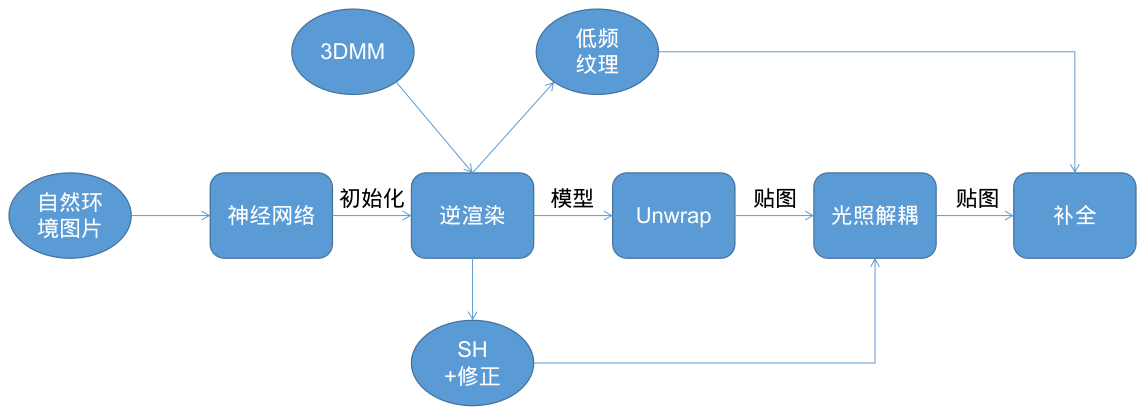
\includegraphics[width=0.95\linewidth]{figures/recon_overall}
    \caption{人脸重建总体流程}
    \label{fig:recon_overall}
\end{figure}

为完成该人脸重建的目标,本方法将输出一个基于预定义的拓扑结构的三角形网格,以及其对应的高清纹理贴图,该图的像素中编码了人脸表面的光线反射率。
其总体流程如\ref{fig:recon_overall}所示。
本文首先利用现有方法\citep{deep3d}根据输入的照片估计3DMM人脸模型的形变系数,环境光照,人脸姿态等信息。
以此作为初始化,本文利用第\ref{chap:method}章提出的方法进一步将模型精确对齐到输入照片中,并进一步优化对环境光照的估计。
然后本文将照片的像素投影到纹理空间,依据估计的环境光照将照片中的光照效果和人脸本身的反射率分离,以支持渲染时的光照变化。
最后,本文利用3DMM建模的低频纹理对模型在照片中被遮挡的部分进行补全,以支持渲染时视角的变化。

后文将对该流程中的每个步骤进行详细介绍。

\section{基于神经网络回归的模型初始化}
\label{sec:recon_init}

基于可微分渲染的逆渲染方法通常难以处理较大的姿态变化,它容易在复杂的非线性优化中陷入局部最优。
因而之前很多方法均使用了2D人脸关键点检测结果以提供大范围的,较为平滑的监督信号。
然而关键的的位置定义是较为模糊的,3D模型上的标注和2D检测的误差都会导致误差传递到之后的步骤中。
而本文则不使用关键点以避免这些传递误差,同时免去模棱两可的3D模型关键点标注工作。
本文提出利用现有神经网络方法\citep{deep3d}通过输入照片估计其中人脸3DMM模型的形变系数,环境光照,人脸姿态等信息,并以此作为下一步骤的初始化。

\paragraph{人脸检测}
具体来说,对于一张输入的照片$\mathcal{I}\in\mathbb{R}^{H\times W\times 3}$,本文首先在其中检测人脸。
在输入前本文首先对照片$\mathcal{I}$进行$N$倍降采样(平均池化)为$\mathcal{I}_m$以控制检测的资源消耗,其中$N=\left\lceil \max(H, W) / 1024\right\rceil$,也就是将最长边控制在1024像素以内。
本文使用了\citet{SFD}开源的人脸检测软件。
该软件能输出矩形人脸检测框,本文选择其输出的面积最大的检测框$B$。

\paragraph{系数预测}
然后本文进一步将照片$\mathcal{I}_m$降采样为$\mathcal{I}_s\in\mathbb{R}^{224\times 224\times 3}$,将检测框包含在其中并使其面积最大且居中。
若裁剪框超出像素边缘则填充黑色,以保持人脸在图像中心。
然后$\mathcal{I}_s$将输入到\citet{deep3d}开源的软件中,
它将输出BFM模型\citep{BFM}的
人脸身份系数$\mathbf{\alpha}_\mathrm{id}\in\mathbb{R}^{80}$,
人脸表情系数$\mathbf{\alpha}_\mathrm{exp}\in\mathbb{R}^{64}$,
人脸纹理系数$\mathbf{\alpha}_\mathrm{tex}\in\mathbb{R}^{80}$,
人脸姿态$\mathbf{M}_\mathrm{d}\in\mathrm{SE(3)}$,
环境球谐光照系数$\mathbf{\gamma}\in\mathbb{R}^{9\times 3}$。
其中涉及到的相机坐标系的3D坐标均可通过约定的投影矩阵$\mathbf{P}_\mathrm{d}$投影回图像平面,并与输入图像$\mathcal{I}_s$较好地对齐。

\paragraph{坐标系转换}
然而,上一步骤预测时使用的投影矩阵是固定的,而输入的照片拍摄时使用的设备,人脸在照片中的尺寸,位置都有不同。
为了获取尽可能精确的结果,本文试图从照片的元数据中提取相机实际参数,结合裁减的方式,计算更准确的投影矩阵,并将所涉及到的3D坐标在不同投影矩阵间进行转换,同时满足:3D点在图像上投影的位置基本不变;人脸模型在3D空间的尺度基本不变。

此处投影矩阵定义为$3\times 3$的矩阵$\mathbf{P}$,其使用方式为$\mathbf{x} = \mathbf{P}\mathbf{X}$,
其中$\mathbf{X}$为相机坐标系下的点的三维坐标,$(\mathbf{x}_x/\mathbf{x}_z,\mathbf{x}_y/\mathbf{x}_z)\in[-1,1]^2$即是该点投影到图像上的二维坐标。
注意此处的图像坐标系与图像分辨率无关,这与OpenGL等渲染库的约定一致,且便于后续在不同投影矩阵转换时的计算。
但与OpenGL中常用的投影矩阵形式不同,为了简化推导,此处的投影矩阵并未投影深度。
可从照片的EXIF中提取的信息包括相机焦距$f\in\mathbb{R}$,分辨率$\mathbf{r}\in\mathbb{R}^2$,传感器像素密度$\mathbf{\rho}\in\mathbb{R}^2$。
根据这些信息,并假设该相机符合完美的小孔成像模型,则该相机的投影矩阵为:
\begin{equation}
    \mathbf{P}_\mathrm{cam} = \begin{bmatrix}
        \frac{2f\mathbf{\rho}_x}{\mathbf{r}_x} & 0 & 0 \\
        0 & \frac{2f\mathbf{\rho}_y}{\mathbf{r}_x} & 0 \\
        0 & 0 & 1
    \end{bmatrix}
    \text{。}
\end{equation}
进一步地,裁减操作可以看作是平移和缩放操作的组合,记裁剪框的左下角和右上角坐标分别为$\mathbf{p}_\mathrm{min},\mathbf{p}_\mathrm{max}\in[-1,1]^2$,
则裁剪框内区域的投影矩阵为:
\begin{equation}
    \mathbf{P}_\mathrm{crop} = \begin{bmatrix}
        \frac{2}{\mathbf{p}_\mathrm{max,x}-\mathbf{p}_\mathrm{min,x}} & 0 & 0 \\
        0 & \frac{2}{\mathbf{p}_\mathrm{max,y}-\mathbf{p}_\mathrm{min,y}} & 0 \\
        0 & 0 & 1
    \end{bmatrix}\begin{bmatrix}
        1 & 0 & -\frac{\mathbf{p}_\mathrm{min,x}+\mathbf{p}_\mathrm{max,x}}{2} \\
        0 & 1 & -\frac{\mathbf{p}_\mathrm{min,y}+\mathbf{p}_\mathrm{max,y}}{2} \\
        0 & 0 & 1
    \end{bmatrix}\mathbf{P}_\mathrm{cam}
    \text{。}
\end{equation}

以下将介绍具体如何将3D模型从投影矩阵$\mathbf{P}_\mathrm{d}$转换到$\mathbf{P}_\mathrm{crop}$下。
该转换分为两步,将模型关于相机旋转以保持模型中心点投影位置不变,再将模型向朝向或远离相机的方向平移以保持模型的投影尺度不变。
这两步操作均为刚性变换,因此可以保证模型在3D空间的尺度不变。

首先求解旋转,该步骤主要用于平衡不同照片中人脸裁剪框位置的差异。
记3D网格模型$M=\{\mathbf{v}_i\}_i$为三维顶点的集合,其中$\mathbf{v}_i\in\mathbb{R}^3$为神经网络预测的顶点的三维坐标。
记$\bar{\mathbf{v}} = \frac{1}{|M|}\sum_{i=1}^{|M|}\mathbf{v}_i$为模型中心点的三维坐标。
若要该中心点的投影位置不变,则该点应位于新坐标系下的一条以原点为起点的射线上,该射线上另一点的坐标为$\bar{\mathbf{v}}' = \mathbf{P}_\mathrm{crop}^{-1}\mathbf{P}_\mathrm{d}\bar{\mathbf{v}}$。
因此,所需旋转的旋转轴为$\bar{\mathbf{v}}' \times \bar{\mathbf{v}}$,
旋转角为$\arccos\left(\frac{\bar{\mathbf{v}}'\cdot\bar{\mathbf{v}}}{\|\bar{\mathbf{v}}'\|\|\bar{\mathbf{v}}\|}\right)$。
可由罗德里格斯公式计算其对应旋转矩阵$\mathbf{R}$,类似公式\ref{eq:rodrigues},此处不再赘述。
旋转后的中心点坐标记为$\bar{\mathbf{v}}'' = \mathbf{R}\bar{\mathbf{v}}$。

然后可以求解所需平移,该步骤主要用于平衡不同相机的焦距参数的差异。
记平移后的中心点位置为$\bar{\tilde{\mathbf{v}}} = s\bar{\mathbf{v}}''$,
$s$表示平移前后该点据相机的距离比例。
若要模型投影尺度不变,则$s$应满足如下方程:对于三维坐标$\mathbf{x}=[x,y,z]^\mathsf{T}$
\begin{equation}
    \left.\nabla_{x,y}\left(\frac{\mathbf{P}_\mathrm{crop}\mathbf{x}}{z}\right)\right|_{\mathbf{x}=\bar{\tilde{\mathbf{v}}}} =
    \left.\nabla_{x,y}\left(\frac{\mathbf{P}_\mathrm{d}\mathbf{x}}{z}\right)\right|_{\mathbf{x}=\bar{\mathbf{v}}}
    \text{。}
\end{equation}
该方程是超定方程,但由于这里使用的投影矩阵均是按相同比例处理x和y轴的,因此应当能解出一致的$s$。在实践中可以使用最小二乘法求解。

在得到针对模型中心点的变换参数后,可将其合成一个变换矩阵以应用到整个模型的任意顶点上。
变换矩阵为:
\begin{equation}
    \mathbf{M}_\mathrm{t} = \begin{bmatrix}
        \mathbf{I} & \bar{\tilde{\mathbf{v}}} - \bar{\mathbf{v}}'' \\
        \mathbf{0} & 1
    \end{bmatrix}\mathbf{R}
    \text{,}
\end{equation}
转换后的模型即为$\tilde{M}=\{\mathbf{M}_\mathrm{t}\mathbf{v}_i\}_i$,其中$\mathbf{v}_i$需在最后一维上加上1以扩展为齐次坐标。
图\ref{fig:crop}用一个玩具实验展示了转换前后的模型,以及该转换的必要性。

\section{模型裁剪边缘的梯度处理}
\label{sec:recon_sdf}

可微分渲染在应用到人脸3D重建时有一个特殊的问题:人是一个很大的物体,而人脸重建的目标通常仅仅是人脸的这一小块区域。
所以通常在人脸重建中用于逆渲染的模型都是裁剪过的,只包含人脸的部分,因此具有一些人为制造的边缘。
这些边缘在照片中并不存在,但第\ref{chap:method}章提出的方法在应用到人脸时却也会在这些边缘产生相关梯度,由于并无对应的边缘可供对齐,这些梯度将导致模型过度扩展,影响最终收敛的效果。

解决该问题的关键在于如何判断渲染图像中的像素与模型指定边缘的位置关系,以便在计算梯度时能够区分人为制造的边缘和真正需要优化的边缘。
对此,本文受到\citet{sdf_glyphs}的启发,该作者提出使用SDF(Signed Distance Field,有向距离场)贴图来绘制可任意放大的矢量图形,并能根据SDF的梯度判断像素到图形边缘的距离,从而实现各向异性的抗锯齿。
于是,本文提出一种简单的基于SDF贴图的方法来区分人为制造的和真正需要优化的边缘。

具体地,本文定义一种SDF贴图。
对于该贴图中的每个像素,其值为一个单通道浮点数$d$,表示该像素点到最近的人为制造边缘的距离,在模型内部的为正,模型外部的为负,
如图\ref{fig:sdf}所示。
由于该贴图中并无太多高频信息,本文仅使用了$256 \times 256$的分辨率。
虽然似乎只有模型内部的贴图像素才会在渲染时被采样到,只需要计算模型内部的正值即可,但实际上,由于采样时使用双线性插值,外部的负值也会被采样到从而参与插值计算中.
更准确的线性插值结果正是SDF的主要优势之一。
从图中也可见,无论是SDF值还是其梯度在穿过边缘时都依然是平滑的。

\begin{figure}
\centering
\begin{subfigure}[t]{3.3in}
    \centering
    \import{build/figures}{sdf.pgf}
    \caption{SDF贴图}
    \label{fig:sdf}
\end{subfigure}
\begin{subfigure}[t]{2.9in}
    \centering
    \import{build/figures}{sdf_grad.pgf}
    \caption{SDF的梯度}
    \label{fig:sdf_grad}
\end{subfigure}
\caption[SDF贴图可视化]{SDF贴图可视化。灰色线为模型中人为制造的边缘。(a)为SDF贴图,表示每个像素到最近边缘的距离,模型内部为正,外部为负;(b)为(a)的梯度向量,其x和y分量分别可视化为红色和绿色通道。}
\end{figure}

下面以nvdiffrast的工作方式为例说明该贴图的使用方式:
nvdiffrast抗锯齿模块工作时将以一对相邻的像素点为单位(如图\ref{fig:aa}),其中一个像素在模型内部,另一个像素在模型外部。
对于处于模型内部的像素,可从SDF贴图中采样其对应的$d$值,并计算$\frac{\partial d}{\partial \mathbf{x}}$,其中$\mathbf{x}$为对应外部像素相对该内部像素的坐标偏移量。
也即对3D模型的表面在该内部像素点的位置使用一个平面进行一阶近似,并求外部像素在该近似平面上的位置,以估计外部像素是否在人为制造边缘之外。
正式地,对于一对分别处于模型内外的像素点,其处于人为制造的边缘当且仅当:
\begin{equation}
    d + \max\left(a\frac{\partial d}{\partial \mathbf{x}}, \delta\right) < 0
    \text{,}
\end{equation}
此时应该忽略其产生的可见性梯度。其中$\delta=0.1$为人为限制的梯度的最大值,为避免小概率时过大梯度产生过于离谱的结果;$a=1.5$为梯度放大的系数,为避免偶发的由于精度不足导致的检测遗漏。
这两个超参数的选择对最终结果的影响不大。

\begin{figure}
\centering
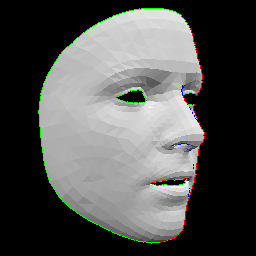
\includegraphics[height=2.2in]{figures/debug_sdf}
\caption[人为制造边缘分类效果]{人为制造边缘分类效果。绿色为人为制造的边缘;红色为与未知背景间的边缘;蓝色为模型内部相互遮挡产生的边缘。}
\label{fig:sdf_result}
\end{figure}

该算法对边缘分类的效果如图\ref{fig:sdf_result}所示。
可见算法将所有边缘分为了三类,
其中绿色为人为制造而需要忽略的边缘,
红色为与未知背景间的边缘,可按照第\ref{chap:method}章提出的方法进行处理,
蓝色为模型内部相互遮挡产生的边缘,应按正常可微分渲染流程处理。
从图中可见一些红色与绿色交错的区域,这是由于这两种边缘本身并没有明确的界限,有时人为制造的边界会正好投影到实际边界附近。
因此本文认为这种现象是十分合理且可接受的。

\paragraph{SDF贴图的计算}
关于SDF的计算方法有很多,下面介绍本文的实现方式。
本文首先使用Blender将3D人脸模型展开至纹理空间,然后在展开后的所有三角形中查找仅属于一个三角形的边做为所谓人为制造的边缘。
并将这些边加入CGAL封装的层次包围盒\footnote{https://doc.cgal.org/latest/AABB\_tree/index.html}数据结构中,以便快速查找。
随后调用OpenGL将所有展开后的三角形光栅化渲染至图像中,得到边缘内部像素的遮罩。
最后,对于贴图中的每个像素,从层次包围盒中查找与其最近的边,计算其与该边的距离$|d|$,并根据遮罩赋予其符号。$d$的梯度方向即为从该像素指向该边上与其最近点的方向(或反方向),模长为$1$。
本方法相比\citet{sdf_glyphs}介绍的暴力方法效率更高,本方法计算$256\times256$分辨率的贴图,使用CPU单线程用时在10毫秒左右。

\paragraph{梯度计算}
梯度$\frac{\partial d}{\partial \mathbf{x}}$的计算与所使用的渲染方式有关。
例如OpenGL支持通过数值方法直接求任意变量关于像素坐标的梯度\footnote{https://registry.khronos.org/OpenGL-Refpages/gl4/html/dFdx.xhtml}。
而针对本文使用的nvdiffrast来说,本文首先以解析法随SDF一同计算其关于纹理坐标的梯度$\frac{\partial d}{\partial u}$和$\frac{\partial d}{\partial v}$,并将其与$d$一同保存于贴图中。
然后根据nvdiffrast的插值模块给出的纹理坐标和像素坐标间的雅可比矩阵将其到像素坐标:
\begin{equation}
    \begin{bmatrix}
        \frac{\partial d}{\partial x} \\
        \frac{\partial d}{\partial y}
    \end{bmatrix} = \begin{bmatrix}
        \frac{\partial u}{\partial x} & \frac{\partial u}{\partial y} \\
        \frac{\partial v}{\partial x} & \frac{\partial v}{\partial y}
    \end{bmatrix} \begin{bmatrix}
        \frac{\partial d}{\partial u} \\
        \frac{\partial d}{\partial v}
    \end{bmatrix}
\text{。}
\end{equation}
该方法与\citet{sdf_glyphs}中提出的方法相同。
所要求的$\frac{\partial d}{\partial \mathbf{x}}$根据前景和背景像素的相对位置,是$\frac{\partial d}{\partial x}$或$\frac{\partial d}{\partial y}$或其相反数四者之一。

另一种解决该问题的可能的方案是屏蔽位于模型表面特定区域的像素上的可见性梯度,例如屏蔽特定三角形,屏蔽到边缘距离小于某个阈值的区域,手动指定遮罩等。
相比于这些方法,本方法具有如下优势:
\begin{enumerate}
\item 渲染尺度无关:同样的模型区域在不同尺度下渲染呈现的尺度不同,因此屏蔽区域的选择可能需要随着尺度变化而改变。
而本方法融入$d$了对像素坐标的梯度信息,是模型表面的一阶近似,因此不受尺度的影响。
\item 有向性:即使是同一个像素,在其不同方向上也可能分别靠近不同种类的边缘。
本方法通过考虑$d$的梯度方向,可以区分这些不同的边缘。
\end{enumerate}

\section{基于可微分渲染的逆渲染优化}

\begin{figure}
\centering
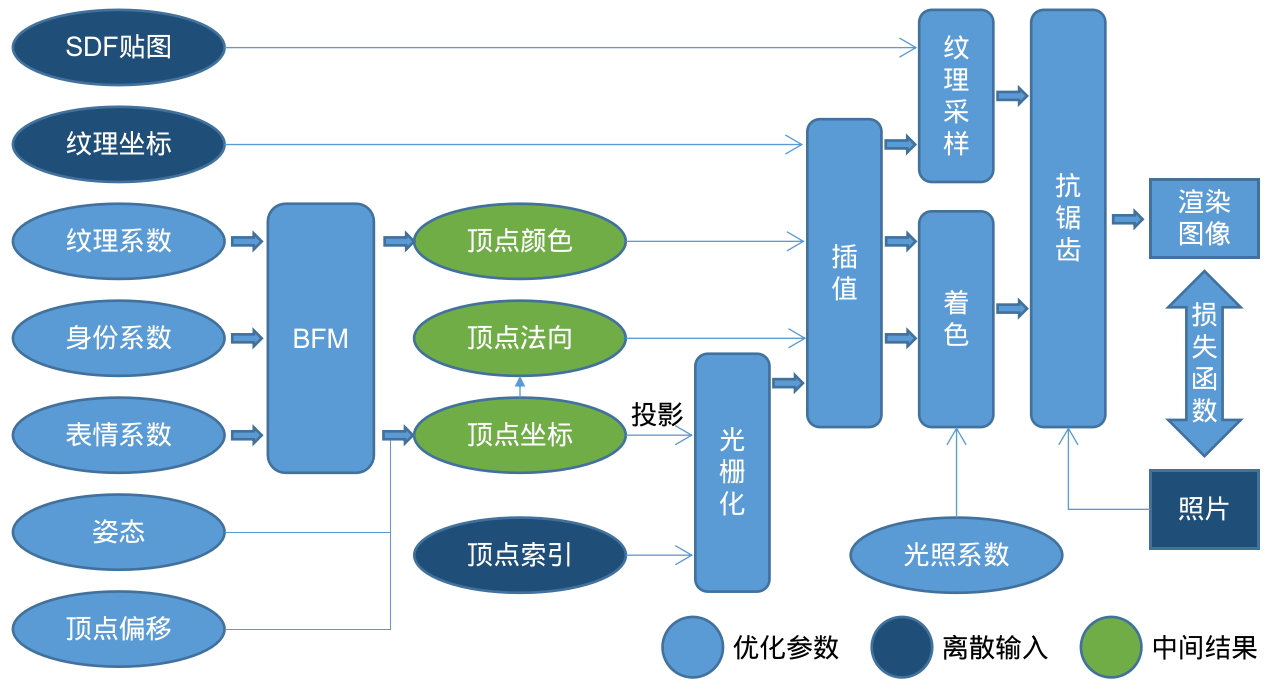
\includegraphics[width=\linewidth]{figures/recon_render}
\caption{渲染的整体流程}
\label{fig:recon_render}
\end{figure}

基于第\ref{sec:recon_init}节计算的3D模型、纹理、环境光照估计作为初始化,
以及第\ref{chap:method}章和第\ref{sec:recon_sdf}节提出的方法,
本节具体将介绍如何将它们结合nvdiffrast\citep{nvdiffrast}实际应用于人脸3D模型的逆渲染过程中。
渲染的整体流程如图\ref{fig:recon_render}所示。
逆渲染的目标即是通过梯度下降优化的方式,优化模型参数,使得渲染结果与照片尽可能接近。
以下将具体介绍该流程中的各个步骤。

\paragraph{顶点计算和投影}
首先本文实现了类似传统渲染引擎中的顶点着色器的计算。
这个步骤输入模型的各种数据和参数,输出该模型每个顶点在裁切空间中的坐标,以及定义在每个顶点上的一些附加属性。
本文由是使用的着色模型较为简单,因此附加属性仅包括法线,反射率和纹理坐标。

首先,本文依据类似3DMM模型的方式计算其每个顶点的位置和反射率:
\begin{align}
\mathbf{S} &= \bar{\mathbf{S}} +
\mathbf{B}_\mathrm{id}\mathbf{\alpha}_\mathrm{id} +
\mathbf{B}_\mathrm{exp}\mathbf{\alpha}_\mathrm{exp} +
\mathbf{S}_\mathrm{off}\\
\mathbf{T} &= \bar{\mathbf{T}} +
\mathbf{B}_\mathrm{tex}\mathbf{\alpha}_\mathrm{tex}
\text{。}
\end{align}
其中$\bar{\mathbf{S}}$和$\bar{\mathbf{T}}$分别是平均的人脸形状和反射率,
$\mathbf{B}_\mathrm{id}$、$\mathbf{B}_\mathrm{exp}$和$\mathbf{B}_\mathrm{tex}$分别是身份、表情和反射率的PCA基,并预先根据其对应的标准差进行了放大。
与之前方法\citep{deep3d,GuoZCJZ19}保持一致,本文使用了BFM 2009模型\citep{BFM}中的身份和反射率基,以及从Face Warehouse\citep{FaceWarehouse}中创建的表情基。
$\mathbf{\alpha}_\mathrm{id}$、$\mathbf{\alpha}_\mathrm{exp}$和$\mathbf{\alpha}_\mathrm{tex}$分别是身份、表情和纹理的系数,是所需优化的参数。
与之前的方法不同,本文使用了\ref{sec:recon_init}节中预测的系数来计算$\bar{\mathbf{S}}$和$\bar{\mathbf{T}}$,从而利用神经网络中的知识作为逆渲染优化的先验。
此外,本文还额外对顶点位置增加了一个偏移量$\mathbf{S}_\mathrm{off}$,以允许其偏离PCA产生的低维空间,拟合更加多样的人脸形状,从而充分发挥逆渲染用于监督的信息量大的优势。

在获得顶点位置后,还需将其变换到相机坐标系并投影到裁切空间中,以便后续的光栅化。投影后顶点在裁切空间中的坐标为:
\begin{equation}
\mathbf{S}_\mathrm{clip} = \mathbf{P}_\mathrm{crop}\mathbf{M}_\mathrm{t}\mathbf{M}_\mathrm{d}\mathbf{M}_\mathrm{c}\mathbf{S}
\text{,}
\end{equation}
其中$\mathbf{M}_\mathrm{c}\in \mathrm{SE(3)}$是可优化的参数。
该步骤在之前第\ref{sec:recon_init}节神经网络预测($\mathbf{M}_\mathrm{d}$)和坐标系转换($\mathbf{M}_\mathrm{t}$)后的结果的基础上,再增加了一个参数以给逆渲染进一步优化的空间。
需注意,此处的投影矩阵$\mathbf{P}_\mathrm{crop}$需要选取合适的近截平面和远截平面,扩展为$4\times 4$的投影矩阵,以将深度也投影在$[-1,1]$范围内,支持下一步光栅化的深度缓冲和深度测试算法。

除了顶点位置和反射率,本文还计算了每个顶点的法线。
通行的做法是根据顶点周围的三角形的形状,对三角形的发现做加权平均。
但由于BFM模型的网格较为密集且均匀,简单起见,本文直接使用了与每个顶点相邻的多个三角形的法线平均值作为该顶点的法线。即第$i$个顶点的法向为:
\begin{equation}
\mathbf{n}_i \propto \sum_{j\in\mathcal{N}_i}\mathbf{n}_{tri,j} \quad
\|\mathbf{n}_i\| = 1
\text{,}
\end{equation}
其中$\mathcal{N}_i$是与顶点$i$相邻的三角形的集合,$\mathbf{n}_{tri,j}$是三角形$j$的法向,可由其三个顶点的坐标求得。
之所以不直接使用每个三角形的法线进行着色(即如图\ref{fig:sdf_result}中的着色效果),
是希望在图像中法线方向是平滑变化的,不会在三角形交界处出现明显的跳变。

\paragraph{光栅化}
光栅化的目的是建立3D网格中的三角形和图像中的像素的对应关系。
该步骤本文直接使用了nvdiffrast中的光栅化模块,
其输入为顶点的裁切空间坐标$\mathbf{S}_\mathrm{clip}$和每个三角形的顶点索引,
输出为每个像素的三角形索引和其在该三角形中的重心坐标$\mathbf{w}$,
以及重心坐标对图像像素坐标的梯度$\frac{\partial\mathbf{w}}{\partial\mathbf{x}}$。

\paragraph{插值}
插值步骤根据光栅化中建立的对应关系,将定义在顶点上的属性(如上述反射率、法线、纹理坐标)插值到像素上,以得到定义在像素上的相同属性。
同时,根据重心坐标对图像像素坐标的梯度,也可以计算出对应的属性梯度。
本文也直接使用了nvdiffrast中的插值模块。

\paragraph{纹理采样}
纹理采样步骤根据上述插值得到的纹理坐标$(u,v)$,从纹理图中获取该坐标下的属性值,以得到定义在像素上的相同属性。
本文同样也直接使用了nvdiffrast中的纹理采样模块。
本文所使用的纹理仅有如第\ref{sec:recon_sdf}节中所描述的SDF贴图。
对该贴图采样过程将得到定义在像素上的距离$d$以及其关于纹理坐标$(u,v)$的梯度$\frac{\partial d}{\partial u}$和$\frac{\partial d}{\partial v}$。

\paragraph{片元着色}
片元着色的目的是根据光照模型和上述各种属性计算每个像素最终的颜色,即其向相机方向反射的光线的能量分布。
本文使用二阶球谐函数(SH)来表示光照,并定义在YUV色彩空间上。该模型每个通道使用9个参数,共27个参数即可近似表示低频环境光照,
具体计算方式是\citet{sh_diffuse}的推导结果的实现。
对于每个像素,其各个方向的总入射光强为:
\begin{gather}
    \begin{aligned}
        \mathbf{E}^\mathrm{sh}_i(\mathbf{n}) &=
        c_1 L_{22}(\mathbf{n}_x^2-\mathbf{n}_y^2) +
        c_3 L_{20}\mathbf{n}_z^2 +
        c_4 L_{00} -
        c_5 L_{20} \\
        &+ 2c_1(L_{2-2}\mathbf{n}_x\mathbf{n}_y +
                L_{21}\mathbf{n}_x\mathbf{n}_z +
                L_{2-1}\mathbf{n}_y\mathbf{n}_z)
         + 2c_2(L_{11}\mathbf{n}_x +
                L_{1-1}\mathbf{n}_y +
                L_{10}\mathbf{n}_z) \\
        \end{aligned} \\
        c_1 = 0.429043 \quad
        c_2 = 0.511664 \quad
        c_3 = 0.743125 \quad
        c_4 = 0.886227 \quad
        c_5 = 0.247708 \notag
        \text{,}
\end{gather}
其中$L$是二阶球谐函数的系数,$\mathbf{n}$插值后归一化的法向量,光强对每个通道$i$分别计算。
具体推导过程较为复杂,感兴趣的读者可参考引用的原论文。
这些参数将使用第\ref{sec:recon_init}节中介绍的神经网络的预测结果初始化,但由于色彩空间和其他定义方式有区别,此处需要进行一些转换。

然而,仅使用球谐函数表示的环境光照是很粗糙的,例如,它作为局部着色方法,无法建模人脸本身的自遮挡现象。
此外,算法估计的人脸几何形状由于3DMM的表达能力有限,也能出现系统性的偏差。
拍摄者使用的相机的gamma校正,相机内建的自动亮度优化等也会对逆渲染产生影响。
这些偏差若不做处理,则最终均会反映到下一节中重建的反射率纹理上,从而影响模型在新环境向的渲染效果。
因此,本文也采用了\citet{IchimBP15}提出的方法,引入一个光照修正场,用于吸收上述所有未能建模的偏差中的低频部分。
但与本文不同,该作者是在纹理空间进行着色计算的,其修正场也是定义在纹理空间。
因此本文选择直接在像素空间定义光照修正场$\mathbf{E}^\mathrm{off}\in\mathbb{R}^{3\times H\times W}$,即照片中每个像素每个通道的入射光强偏差。

着色时本文仅考虑了朗伯特漫反射模型,即反射光强正比于总入射光强,其比例则直接建模为上述反射率$\mathbf{\rho}$。
因此每个像素最终着色的结果为:
\begin{equation}
    \mathbf{C} = \mathbf{\rho} \left(\mathbf{E}^\mathrm{sh} + \mathbf{E}^\mathrm{off}\right) \text{。}
\end{equation}

\paragraph{抗锯齿}
本文的方法基于nvdiffrast中的抗锯齿模块。
在该实现中,抗锯齿除了能得到观感更好的图像,其最主要的作用是在反向传播时计算物体间相互遮挡造成的可见性相关梯度。
本文对nvdiffrast中的抗锯齿模块进行了较多修改,
其中包括第\ref{chap:method}章中介绍的应对未知背景计算梯度的方法,
第\ref{sec:method_discuss}节中介绍的应对nvdiffrast梯度稀疏的缓解措施,
以及第\ref{sec:recon_sdf}节中介绍的使用SDF贴图对边缘分类的方法。
作为本章最有特色的部分,在无需人脸关键点监督的情况下,本文借助抗锯齿模块提供的可见性梯度实现了人脸模型和具有未知背景的照片的精确对齐。

\paragraph{损失函数}
总结来说,本章通过逆渲染优化的参数包括:
3DMM系数$\mathbf{\alpha}_\mathrm{id}$、$\mathbf{\alpha}_\mathrm{exp}$、$\mathbf{\alpha}_\mathrm{tex}$,
每顶点偏移量$\mathbf{S}_\mathrm{off}$,
人脸姿态$\mathbf{M}_\mathrm{c}$,
以及球谐光照参数$\mathbf{L}$。

为了优化这些参数,本文通过梯度下降的方法优化如下损失函数:
\begin{equation}
    \mathcal{L} = \mathcal{L}_\mathrm{n} + \mathcal{L}_\mathrm{reg}
    \text{,}
\end{equation}
其中$\mathcal{L}_\mathrm{n}$第\ref{chap:method}章中介绍的面积归一化的像素损失,并使用了第\ref{sec:method_discuss}节中介绍的实现方法。
本章中不仅使用了第\ref{chap:method}章中主要介绍的可见性梯度,
还根据本节中介绍的渲染流程计算了着色的梯度。
$\mathcal{L}_\mathrm{reg}$则是正则化项,包括:
\begin{equation}
\begin{split}
\mathcal{L}_\mathrm{reg} = \alpha_1\left(\| \mathbf{\alpha}_\mathrm{id} \|_2^2 +
    \| \mathbf{\alpha}_\mathrm{exp} \|_2^2 +
    \| \mathbf{\alpha}_\mathrm{tex} \|_2^2\right) +
    \alpha_2 \| \mathbf{S}_\mathrm{off} \|_F^2 +
    \alpha_3 \mathcal{L}_\delta +
    \alpha_4 \| \mathbf{L}_{UV} \|_2^2 \\
    + \alpha_5 \| \mathbf{E}^\mathrm{off} \|_F^2 +
    \alpha_6 \| \nabla_{x,y} \mathbf{E}^\mathrm{off} \|_F^2
    \text{,}
\end{split}
\end{equation}
其中第一项是3DMM系数的正则化项,该项使3DMM的结果保持在其先验分布范围内;
第二项约束顶点偏移量的大小,避免模型过度偏离3DMM的预测;
第四项使环境光照更趋向于白色,从而鼓励模型使用反射率参数来解释照片中的颜色;
最后两项分别约束光照修正场和其梯度的大小,限制其强度和频率;
第三项是拉普拉斯正则项,它使模型顶点间的相对位置和拓扑结构在优化过程中保持稳定,其定义为:
\begin{equation}
    \mathcal{L}_\delta = \sum_{i=1}^N \left\|\mathbf{S}_\mathrm{off}^i - \frac{1}{|\mathcal{N}_i|}\sum_{j\in\mathcal{N}_i} \mathbf{S}_\mathrm{off}^j\right\|_2^2
    \text{,}
\end{equation}
其中$\mathcal{N}_i$是与顶点$i$相邻的顶点集合,在实践中可使用稀疏矩阵来实现。
注意此处拉普拉斯正则项的定义与常见的不同,这里直接以偏移量而不是顶点坐标作为输入,因此其形式更加简单;
且并未对不同顶点加权或考虑旋转不变性等,因为本文使用的模型通常顶点分布较均匀,且在3DMM模型建模了绝大部分形变,偏移量总体较小。实践中这种简单的算法即可发挥期望的效果。

通过对以上损失函数的优化,本文实现了人脸模型和具有未知背景的照片的精确对齐,即获得了较为准确的人脸模型几何形状。
并且也得到了对环境光照较为准确的估计。
但由于所使用的反射率信息是来自3DMM的低维空间,其表达能力较弱,不能准确建模人脸的纹理细节。

\section{照片到纹理空间信息迁移}
\label{sec:method_photo2tex}

本节将介绍如何将照片中的信息迁移到人脸模型的纹理中,并计算高分辨率的反射率纹理贴图。
该步骤总体上类似于一次反方向的光栅化渲染过程。
即以照片作为纹理,顶点在裁切空间的坐标作为纹理坐标,而原来的顶点纹理坐标则作为新的裁切空间坐标,进行一次光栅化和插值。
在片元着色阶段,则从照片中以纹理采样的方式获得最终反射进相机的能量分布,在依据预测的环境光照解算出反射率,即$\mathbf{\rho}_\mathrm{img} = \mathbf{C} / \mathbf{E}$。
具体实现方式与正向过程类似,但有几点需注意:
\begin{itemize}
\item 在OpenGL的约定中,裁切空间的坐标范围为$[-1,1]$,而纹理坐标为$[0,1]$,因此它们在交换时需要分别进行一次线性变换以映射到正确的范围;
\item 在对原裁切空间坐标进行插值以获得新的纹理坐标时,需要对齐次坐标进行插值,再除以插值后的$w$坐标,而不能反过来处理,如此才能获得透视变换正确的插值结果。
图\ref{fig:unwrap_interpolate}展示了这两种不同操作顺序到的的不同结果。
\end{itemize}

此外,人脸在特定视角下只能观测到其未被遮挡的部分,因此以上述方法渲染出的纹理图像中,只有映射到照片中可见表面的部分才是有效的。
为识别出这些有效的纹理区域,本文使用了如下两个策略:
\begin{enumerate}
\item 将上述计算的每个顶点的3D坐标$\mathbf{v}$和法向$\mathbf{n}$也插值到渲染出的纹理空间中,则法向与相机方向的夹角超过90°的像素所在表面是背向相机的,可认为是无效区域。
\item 先以正常照片的视角渲染一张深度图,其中记录照片中的每个像素到相机的距离。然后将该深度图与照片一起,作为纹理采样至新纹理空间。若采样获得的深度值和使用顶点3D坐标计算的深度值相差超过一个阈值,则认为该像素所在位置被其他物体表面遮挡,是无效区域。
\end{enumerate}
这两个策略各有优劣:
前者可准确识别有效和无效区域交界的位置;且法向与相机方向夹角越大其纹理分辨率越低,这也可以为后续补全的步骤提供依据,允许解算的纹理和补全的纹理间平滑过渡。
但该策略则无法区分朝向相机但被遮挡的部分。
后者则可以识别出被遮挡的区域,但由于数值计算的精度有限,需要设定阈值,因此无法准确判别交界的位置。
本文选取两种策略识别的有效区域的并集作为最终的有效区域。
如图\ref{fig:unwrap_result}展示了迁移的结果以及这两种策略的识别效果。

\paragraph{纹理补全}
由于本应用中以不同视角渲染的需求较低本文仅使用了简单的策略对纹理中无效区域进行补全。
本文将3DMM预测的低频纹理与从照片中解算的纹理加权平均,其权重与法向与相机方向夹角的余弦相关:
\begin{equation}
\mathbf{\rho}_\mathrm{fused} = \begin{cases}
    \alpha \mathbf{\rho}_\mathrm{img} + (1-\alpha) \mathbf{\rho}, \alpha = \frac{\mathbf{v}\cdot\mathbf{n}}{\|\mathbf{v}\|} & \text{if像素位于有效区域} \\
\mathbf{\rho} & \text{otherwise}
\end{cases}
\label{eq:texture_fusion}
\end{equation}

最终,通过逆渲染的优化过程,即可获得所需的3D模型顶点坐标$\mathbf{S}$和其纹理$\mathbf{\rho}_\mathrm{fused}$。
该过程中得到的人脸姿态和环境光照信息也可以用于下游的渲染等认为中。

\section{实验结果}

\section{局限性}

本章介绍的方法仅使用了少量建模在3DMM中的人脸先验知识,该信息中不包括人脸的几何和纹理细节。
而基于单张图片同时估计几何和纹理的问题是高度非适定的,因此本文也无法准确地重建这些细节。
目前,本文仅能重建较为低频的几何细节,此外未能表示的细节则全部会烘焙在反射率的纹理中。
这种方式虽然在原始视角和光照条件下渲染时可充分还原照片,但在大幅度改变视角或光照条件时,则会出现明显失真。

此外,本文所使用的简单的朗伯特反射模型也过于简化,无法建模镜面反射导致的高光,以及人脸的次表面散射现象。
这同样会导致在改变视角或光照条件时,渲染出的结果出现失真。


{
\backmatter
\chapter{结论与展望}
\label{chap:conclusion}

本文研究了基于非受限环境照片的3D人脸重建的问题,
提出了一种基于可微分渲染的3D人脸重建算法。
在此之上,本文最终实现了一个完整的人脸重建流程,并取得了较为令人满意的效果。
本文的主要贡献可概括如下:
\begin{enumerate}
\item 本文提出并实现了一种适应未知背景的可微分逆渲染方法,
其中包括了一种面积归一化的像素损失函数,及其基于nvdiffrast的高效实现。
该方法充分利用可见性梯度,能有效将人脸模型对齐到照片中的边缘,并有应用到其他领域的潜力。
\item 本文实现了一个完整基于单张非受限环境照片的人脸重建流程,
在上一点的基础上,本文消除了其应用于人脸模型时的异常梯度。
本文还结合了传统算法以重建纹理细节,实现了鲁棒且自动的3D人脸重建,
并展示了其重建精度和重新渲染的效果。
\end{enumerate}

虽然在限定的范围内,本文取得了较为令人满意的重新渲染效果,
然而还需要看到,相比于业界的先进方案,本文所述的内容在3D人脸重建的应用领域内尚处于蹒跚学步的阶段,
距离真正影视级的工业应用依然较远,还有大量的问题需要解决:
\begin{enumerate}
\item 如何利用高质量的影视级人脸模型来补充高效重建算法的训练数据,从而改善其细节渲染效果,这依然是前沿的研究领域。
新兴的扩散模型与3D人脸模型的结合可能是一个有前景的研究方向。
\item 尽管已经取得了不错的几何精度,本文尚只利用了较为简单的3DMM模型作为先验知识。
本文偶尔会重建出明显不合常理的人脸形状,
更为复杂的以非线性模型建模的人脸先验或能在与逆渲染方法相结合时展现更好的效果。
这也有待进一步探索。
\item 本文所实现的基于单张非受限环境照片的人脸重建流程仍是基于非常基础的渲染模型,
该模型并不能建模镜面反射,次表面散射等较为复杂的光线传播现象。
这导致本文重建的模型仅能在与照片中较为相似的环境光照和视角下重新渲染。
若要实现在影视中的大范围光照和视角变化,则需要有更多参数的更复杂的模型,也意味着需要更高质量的先验知识来重现一些微妙的效果。
\end{enumerate}

展望未来,为更好地建模人脸的先验知识,神经网络等人工智能技术将必不可少。
由于可微分渲染技术的发展应用,3D人脸重建和计算机图形学的关系也愈发密切。
然而计算机图形学独立于人工智能技术已经有了很长的历史,自身已经有了丰厚的技术积累,
笔者的硕士生涯太短,尚未能在这方面有足够的理解和实践。
未来这两个方向的研究者们或许应该加强交流合作,以进一步提升3D人脸模型的制作效率,降低成本。

% 2001年,长篇小说《刀剑神域》面世,其中展示了作者对2022年的科幻设想。
% 故事中人们使用名为“NERvGear”的小型民用终端即可以自身真实形象进入VR游戏中。
% 《刀剑神域》及其同名动画给笔者留下了深刻的印象,
% 如今2022年已过,希望我们也能早日在现实中见证这样的科技。

\bibliography{main}

\hideinblind{
\chapter{致谢}

研究生三年的时光转瞬即逝。
这三年来,我虽有遗憾,但更多的是收获和成长,并度过了一段充实的学生生涯。
相比三年前,我在知识的深度和广度上均有提升,
我深知,这是在导师的指导和同学,以及其他一些人的帮助下才能实现的,我向他们表示感谢。
我首先要感谢我的导师杜卿老师,她温柔耐心、循循善诱,她也对本文的写作给予了很多的建议。
我还要感谢谭明奎教授,他在我的研究方向尚不明朗时为我提供了很多建议和帮助。
谭教授也为我们创造了舒适的实验室环境,并提供了高性能的机器学习计算资源。
特别要感谢CVTE和王乃洲博士,本文的工作也是华南理工大学与CVTE合作项目的成果,
CVTE为本文的所有实验提供了经济支持。
同时,我要感谢我的同学们,与他们相处我感到很快乐,他们也给予了我很多的帮助。
最后,感谢强盛的祖国,和平的时代,富饶的社会,以及无数为之而奋斗的先辈们,所有人的努力造就了今天令人安心的科研环境。
}% end hideinblind

\chapter{攻读硕士学位期间取得的研究成果}

一、已发表(包括已接受待发表)的论文,以及已投稿、或已成文打算投稿、或拟成文投稿的论文情况:

\noindent\begin{tabularx}{\textwidth}{| p{0.5cm} | X | p{1.8cm} | p{1.7cm} | p{1.8cm} | p{1.8cm} |}
\hline
\textbf{序号} & \textbf{发表或投稿刊物/会议名称} & \textbf{作者} & \textbf{发表年份} & \textbf{与学位论文哪一部分相关} & \textbf{被索引收录情况} \\
\hline
 & & & & & \\
\hline
\end{tabularx}

\vskip 0.5cm

二、与学位内容相关的其它成果(包括专利、著作、获奖项目等):

}% end backmatter

\end{document}
